\chapter{Размещение базовых станций БШС для покрытия линейной территории}\label{chapter_linear_network}
% \chapter{Математические модели синтеза топологии сети для охвата линейного участка в виде задачи целлочисленного линейного программирования}\label{chapter_ilp_model}

В данной главе представлены математические модели синтеза топологии БШС. Рассматриваются задачи оптимального размещения базовых станций, максимизирующее телекоммуникационного покрытия вдоль линейного участка. Под линейным участком подразумевается территория вдоль протяженнего объекта, которую необходимо покрыть БШС. Примерами таких объектов могут являться: автомобильные и железные дороги, тоннели метрополитена, магистральные нефте- и газопроводы. 

\section{Актуальность внедрения БШС для телекоммуникационного покрытия линейного участка}

% \begin{itemize}
%   \item Сеть вдоль дорог;
%   \item Сеть вдоль железных дорог;
%   \item Сеть внутри метрополитена;
%   \item Сеть на месторождении.
% \end{itemize}

Эффективным способом повышения технико-экономических показателей при проектировании БШС является оптимизация ее топологии, а именно решение задачи выбора оптимального набора базовых станций. В этой главе представлена задача, в  которой необходимо обеспечить максимальное телекоммуникационное покрытие для охвата протяженного линейного участка. 

Цифровая трансформация не обошла стороной транспортную отрасль. Весь мир активно участвует в развитии интеллектуальных транспортных систем (ИТС).  Создание современной инфраструктуры передачи мультимедийной информации: голос, данные, видео вдоль протяженных магистралей является одной из важнейших проблем при создании новых и функционировании существующих транспортных магистралей \cite{Vish2015}. Одним из перспективных направлений  является организация на транспортных участках автомобильных сетей (Vehicular ad hoc network, VANET) \cite{Massobrio2020, Campolo2015} (Рисунок \cref{fig:part2_roadisdeunit}). VANET позволяет объединить транспортные средства для обмена друг с другом(vehicle-to-vehicle, V2V) и с инфраструктурой (vehicle-to-infrastructure, V2X). 

Развертывание и развитие сетей беспроводной связи
вдоль протяженных магистралей требует решения ряда сложных организационно-технических задач в условиях жестких ограничений на использование частотных, экономических и аппаратных ресурсов. В связи с этим возрастает актуальность решения проблемы оптимального размещения базовых станций вдоль транспортных магистралей, являющаяся одной из важнейших при проектировании БШС этого класса \cite{Vish2015}. 

Организации БШС вдоль автодорог посвящено ряд зарубежных и отечественных работ. Большинство работ касаются проблемы размещения придорожных объектов (Roadside Unit, RSU) или БС вдоль автодорог. В \cite{Cavalcante2012, KHireddine2020} предложены модели, использующие генетический алгоритм для решения задачи о максимальном покрытии. Максимизация покрытия БШС с учетом ограничения стоимости БС представлена в работах \cite{BenBrahim2014, Vishnevsky2016_optimization}. В работах \cite{Liu2014, Gao2018, Jalooli2019} предложены новый модели размещения БС с учетом характеристик трафика на дорожных участках. В \cite{Reis2014} Рейз А. и др. представили задачу размещения БС для протокола IEEE 802.11p/Wave, позволяющая организовать связь для объектов движущихся на скоростях до 200 км/ч.   В \cite{Guerna2021} для задачи развертывания узлов RSU вдоль автодорог представили модель на основе муравьиного алгоритма, максимизирующую телекоммуникационное покрытие. В работах \cite{Cavalcante2012, Liu2017} в качестве ограничений учитываются временные ограничения при размещении БС. В \cite{Bao2018} предлагают жадный алгоритм для минимизации RSU c условием ограничения задержек между любыми двумя узлами сети. В \cite{Mavromatis2019} предложен алгоритм развертывания RSU вдоль дорог сети миллиметрового диапазона, максимизирующий покрытие и учитывающий ограничение по показателю уровня принимаемого сигнала. В работе \cite{Chirkova2020} представлена модель эгоистичного выбора базовых станций в беспроводной сети в игровой постановке, где каждый игрок стремится увеличить свою величину отношения «сигнал к интерференции плюс шум». В работе \cite{Ivanov2018} представлены задача размещения RSU вдоль линейного участка протяженной автомагистрали в виде модели ЦЛП.

\begin{figure}[ht]
  \centerfloat{
      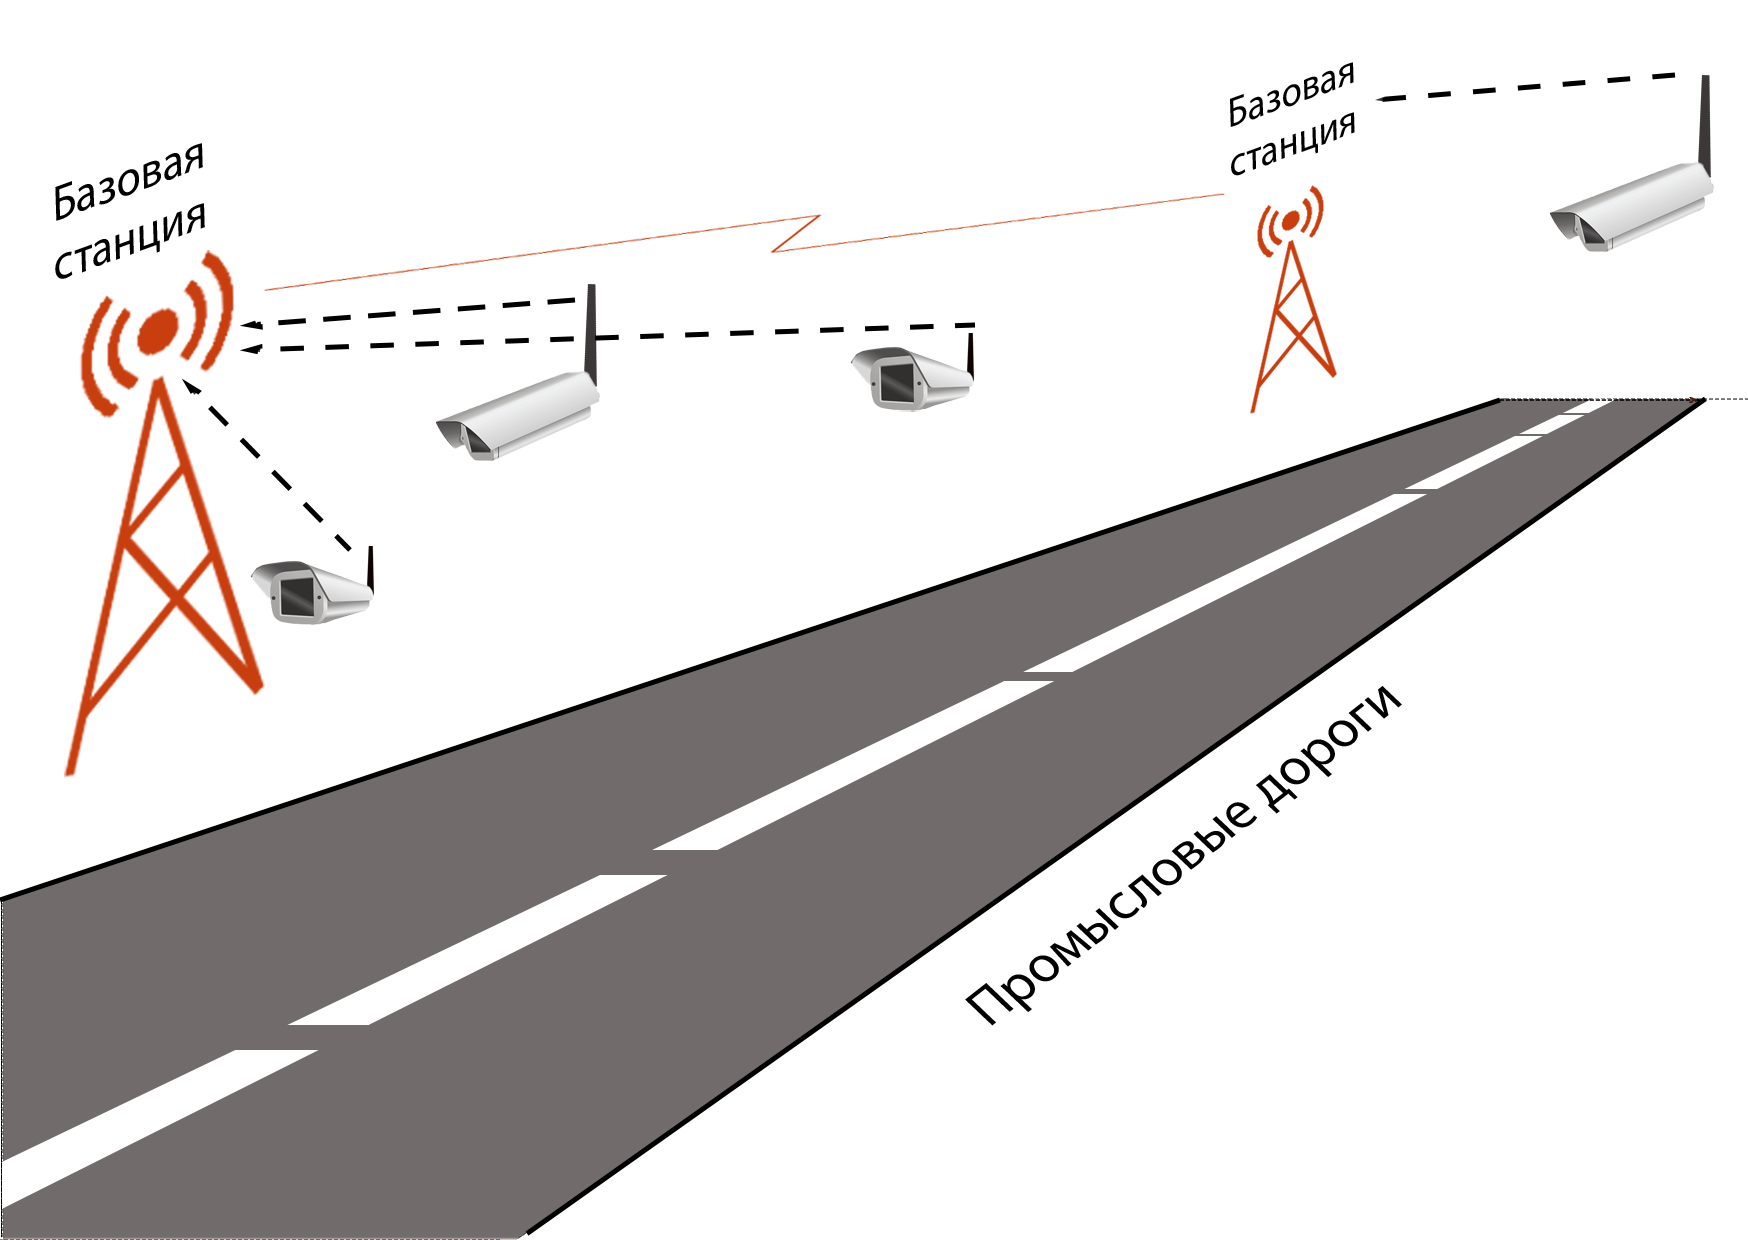
\includegraphics[scale=1.1]{roadsideunit.png}
  }
  \caption{Беспроводная сеть вдоль автомобильных дорог}\label{fig:part2_roadisdeunit}
\end{figure}

\fixme{==========================================}

В нефтегазовом секторе страны сегодня можно отметить резкий тренд цифровизации. Внедрение современных информационных технологий в производственные процессы в рамках перехода к <<Индустрии 4.0>> является главным перспективным направлением зарубежных и отечественных компаний. Данное требование подразумевает рост большого объема данных, требующих современных и надежных телекоммуникационных средств связи. Большинство объектов нефтегазовой отрасли в России охватывают огромные площади и находятся на удалении в труднодоступных регионах, поэтому наилучшим способом организации связи является внедрение БШС. 

Ключевым объектом на нефтегазовом промысле, для которого можно развернуть БШС с линейной топологии, являются магистральные и промысловые трубопроводы, предназначенные для транспортировки товарной нефти или газа из района промысла, производства до места потребления. В общем случае под местами потребления понимают нефтебазы, перевалочные базы, пункты налива в цистерны и заводы \cite{Deineko2018} (Рисунок \ref{fig:part2_pipeline}). В зависимости от географических особенностей и климатических условий магистральные трубопроводы могут прокладываться в подземном, наземном или надземном типах. Перед производством стоит задача не только сбора данных технологического процесса системами автоматизации, но и обеспечение норма безопасности и экологического контроля прилежащей территории. 

\begin{figure}[ht]
  \centerfloat{
      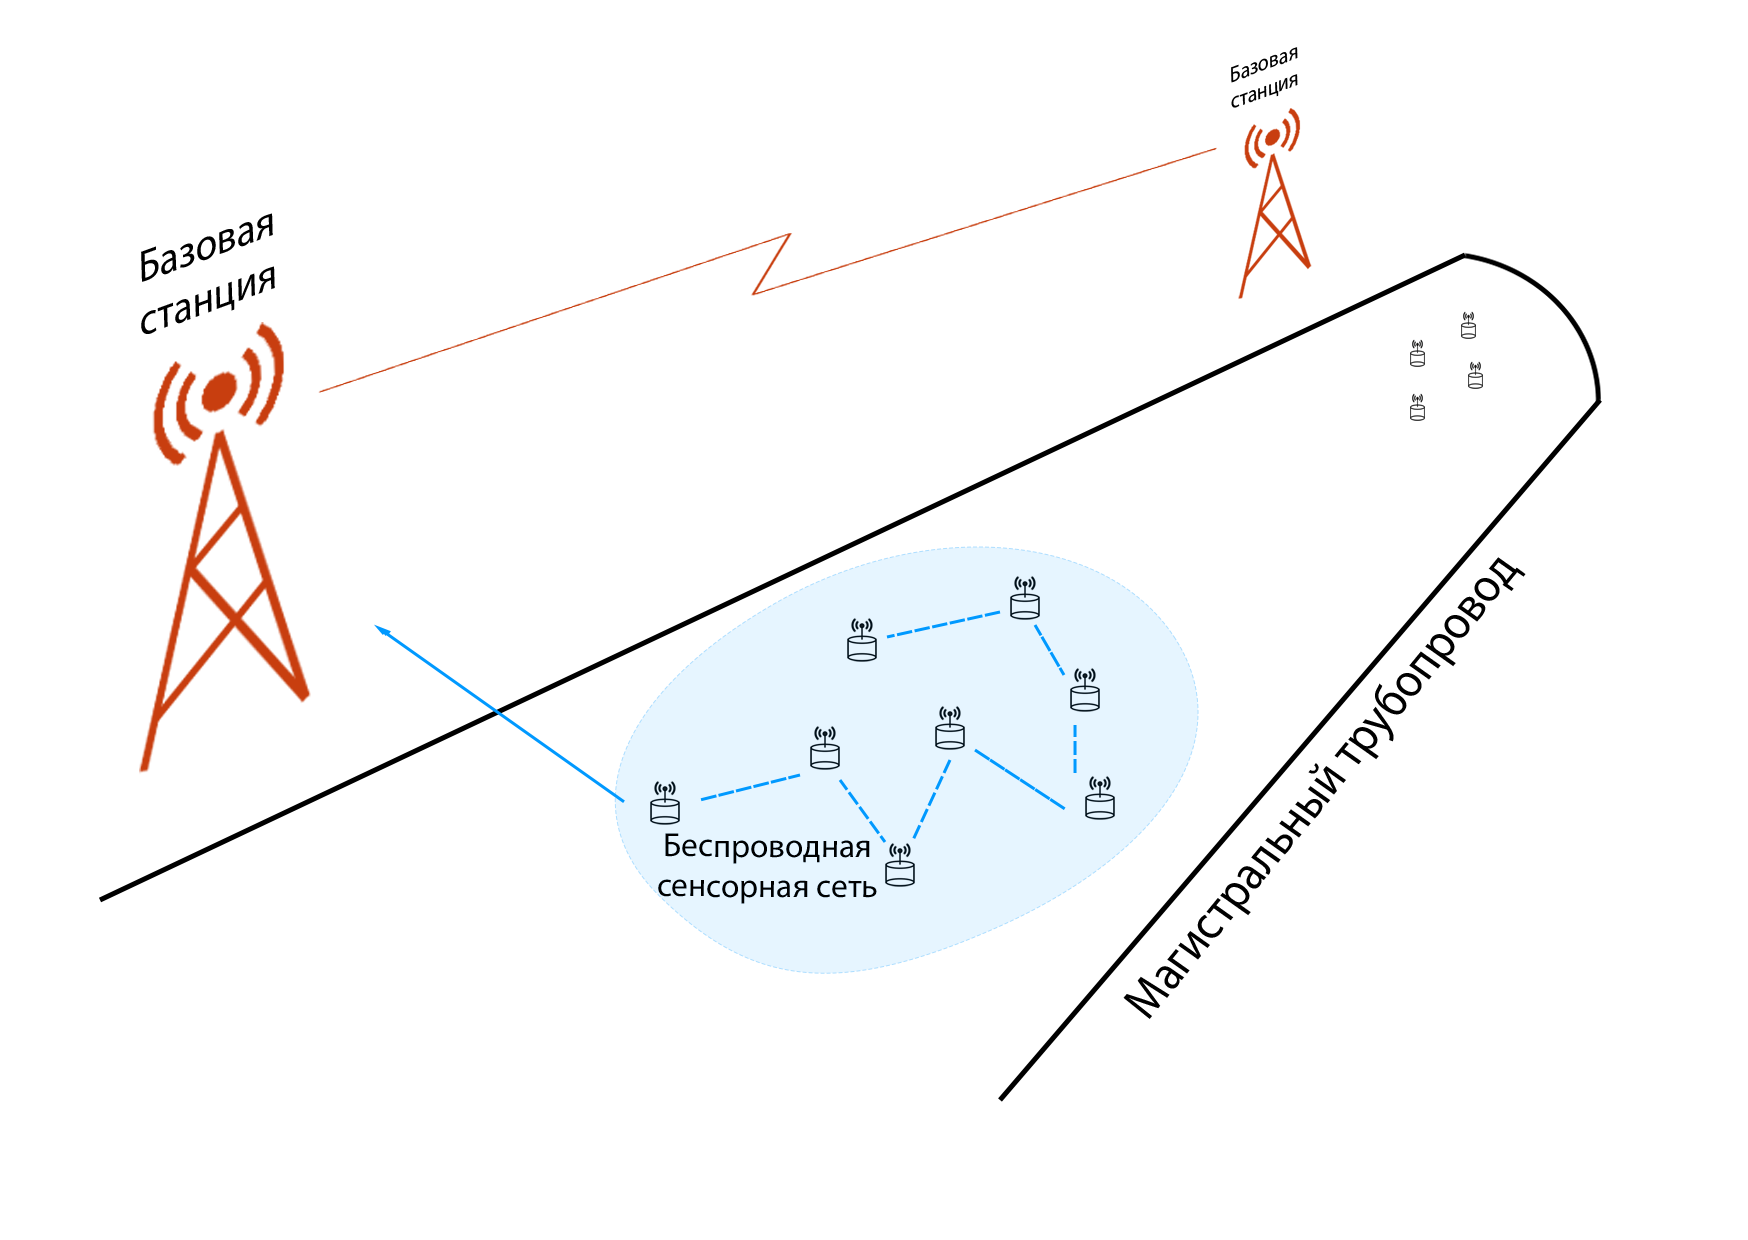
\includegraphics[scale=1.1]{pipeline.png}
  }
  \caption{Беспроводная сеть вдоль нефте- и газопопроводов}\label{fig:part2_pipeline}
\end{figure}

Трубопроводы являются самым безопасным способом транспортировки нефти. К сожалению, одной из главных проблем при таком выборе транпортировке являются случайные утечки. Так к особо уязвимым участкам трубопроводной инфраструктуры относятся регулирующая арматура, ловушки для скребков, приемники скребков, счетчики и манометры. Позднее или несвоевременное обнаружение утечек для нефтегазовой компании  может нанести миллионы финансовых убытков, а также нанести ущерб окружающей среде. В работе \cite{Fawzi2019} представлена интеллектуальная система мониторинга за магистральными трубопроводами в реальном времени с помощью БШС, способной обнаруживать акты вандализма в трубопроводной системе 


Сегодня обеспечение безопасности персонала это задача, которая включает безопасность не только в течение рабочего процесса на технологических объектах, непосредственного, но и в течение всего времени нахождения на промысле. 


Также одним из направлений цифровизации месторождений является внедрение высокоскоростных локальных сетей для организаций связи для мобильных обходчиков. \fixme{Доделать}


Эффективным средством прогнозирования и предотвращения аварийных ситуаций на магистральных трубопроводах, экологической защиты, а также  достижения промышленной безопасности является мониторинг нефтепровода, с помощью современных беспроводных сетей связи, включающие беспроводное технические средства для диагностики состояния трубопроводов, изменений, происходящих под влиянием геологических процессов на опасных участках \cite{Krzyszton2021,Mehmood2016, Lin2019, Adegboye2019, Lin2019}. 

\fixme{=======================================}




Еще одним примером развертывания БШС для охвата линейного объекта является организация телекоммуникационного покрытия на линиях метрополитена \cite{Alekseev2021, radwin_moscow_metro, Soykin2020,aderkina2020, aderkina2021}. Компания Radwin развернула свои базовые станции в тоннелях московского метро, использующий проприетарный протокол передачи данных Wi-Fi 5ГГц \cite{radwin_moscow_metro, Soykin2020}. Оценка нагрузки сети Wi-Fi в московском метро \cite{Alekseev2021}. В работах \cite{aderkina2021, aderkina2020} авторы представили свою эмпирическую модель распространения сигнала, учитывающая отражения в тоннелях, и представили свой алгоритм расстановки базовых станций внутри тоннеля. Основными критериями размещения являются минимизация средней плотности БС и обеспечение уровня принимаемого сигнала не ниже заданного порога при любом расположении состава в тоннеле. Модель распространения основывается на методе геометрической оптики и учитывает как геометрические, так и физические характеристики стен тоннелей. 






\fixme{========================================================================}


 
% Ключевым объектом на нефтегазовом промысле, для которого можно развернуть БШС с линейной топологии, магистральный трубопровод. Магистральные трубопроводы предназначены для транспортировки товарной нефти или газа из района промысла, производства до места потребления. В общем случае под местами потребления понимают нефтебазы, перевалочные базы, пункты налива в цистерны и заводы \cite{Deineko2018}. В зависимости от географических особенностей и климатических условий магистральные трубопроводы могут прокладываться в подземном, наземном или надземном типах. Трубопроводы являются самым безопасным способом транспортировки нефти. К сожалению, одной из главных проблем при таком выборе транпротировке являются случайные утечки. Так к особо уязвимым участкам трубопроводной инфраструктуры относятся регулирующая арматура, ловушки для скребков, приемники скребков, счетчики и манометры. Позднее или несвоевременное обнаружение утечек для нефтегазовой компании  может нанести миллионы финансовых убытков, а также нанести ущерб окружающей среде.

% Одной из главных причин появления аварийных ситуаций на линейных участках трубопровода являются: коррозионные разрушения, механические повреждения при строительстве и эксплуатации, а также заводские браки \cite{Deineko2018_alone}. Для решений данной проблемы возникает важная задача, с которой сталкивается промысел -- отслеживание состояния трубопроводов, по которому транспортируются нефть и газ \cite{Aalsalem2018}. Эффективным средством прогнозирования и предотвращения аварийных ситуаций на магистральных трубопроводах, экологической защиты, а также  достижения промышленной безопасности является мониторинг нефтепровода, с помощью современных беспроводных сетей связи, включающие беспроводное техничекие средства для диагностики состояния трубопроводов, измененений, происходящих под влиянием геологических процессов на опасных участках \cite{Krzyszton2021,Mehmood2016, Lin2019, Adegboye2019, Lin2019}. 

% Наряду с использованием средств промышленной автоматизации в настоящее время свое широкое внедрение получили системы видеонаблюдения с помощью беспилотных летательных аппаратов  (БПЛА, Unmanned Aerial Vehicle, UAV), позволяющие производить мониторинг трубопровода на всем участке в реальном времени \cite{Fedorova2020, Aljuaid2020, Adegboye2019, Gomez2017, Fawzi2019}.

% Одним из интересных направлений в области исследований по обнаружению утечек, отслеживания границ и направления движения токсичных газов является использование мобильных беспроводных сенсорных устройств \cite{Krzyszton2021}. Также одним из направлений цифровизаций месторождений является внедрение высокоскоростных локальный сетей для организаций связи для мобильных обходчиков. 


% до сих пор  невозможно избежать случайных утечек.  Так к особо уязвимым участкам трубопроводной инфраструктуры относятся регулирующая арматура, ловушки для скребков, приемники скребков, счетчики и манометры.
% Хотя утечки в трубопроводе часто начинаются с малого, позднее обнаружение и идентификация утечек может иметь пагубные последствия. Для нефтегазовой компании несвоевременное обнаружение может нанести миллионы финансовых убытков, а также нанести ущерб репутации и окружающей среде.

% Основными причинами аварийных ситуаций на линейных участках являются: коррозионные разрушения, механические повреждения при строительстве и эксплуатации, а также заводские браки \cite{Deineko2018_alone}. Для решений данной проблемы возникает важная задача, с которой сталкивается промысел -- отслеживание состояния трубопроводов, по которому транспортируются нефть и газ \cite{Aalsalem2018}. Эффективным средством прогнозирования и предотвращения аварийных ситуаций на магистральных трубопроводах, экологической защиты, а также  достижения промышленной безопасности является мониторинг нефтепровода, с помощью современных беспроводных сетей связи, включающие беспроводное техничеких средства для диагностики состояния трубопроводов, измененений, происходящих под влиянием геологических процессов на опасных участках \cite{Krzyszton2021,Mehmood2016, Lin2019, Adegboye2019}. В настоящее время свое широкое внедрения получили системы видеонаблюдения, в том числе с помощью БПЛА, позволяющие контролировать безопасность на всем участке трубопровода \cite{Fedorova2020, Aljuaid2020, Adegboye2019, Gomez2017, Fawzi2019}.


% Еще одним из интересных направлений в области обнаружения утечек, отслеживания границ и направления движения токсичных газов является использование мобильных беспроводных сенсорных устройств \cite{Krzyszton2021}. В работе \cite{Lin2019} предлагается беспроводная сенсорная сеть для мониторинга утечек вдоль подземных трубопроводов. 


% На данный момент самым широко используемым классом БШС в нефтегазе являются беспроводные сенсорные сети. Такие сети узлы автоматизации  объедены в низкоскоростную сеть для передачи технологических данных на диспетчерский уровень управления. Хоть беспроводные сенсорные сети уже нашли свое широкого применение, все еще существуют ряд проблем при их развертывании: вероятность потери сигнала при передаче между сенсорами на дальних расстояниях, отказы узлов и проблемы с энергопотреблением, особенно для линейной топологии \cite{Lee2020}. К существенным минусам беспроводных сенсорных сетей можно отнести то, что большинство используемых методов маршрутизации не предназначены для линейной топологии \cite{Abbas2018}. В простейшем случае, когда отказывает один узел, вся сеть перестает функционировать. В силу ограничения на дальности связи передачи данных  целесообразно объединять такие сенсорные сети в кластеры. Для сбора данных с сенсорной сети вдоль линейного объекта используются узлы транспортировки сети -  базовые станции \cite{Fataliyev2018}. Данные с таких классов уже передавать через системы размещенных базовых станций, размещенных вдоль линейного сооружения, беспроводной сети дальнего радиуса действия на базе семейства протоколов IEEE 802.11 (Рисунок \ref{fig:part2_pipeline}).  В \cite{Li2020, Albaseer2019} предложен модели кластеризации узлов БШС. Использование базовых станций в сенсорных сетях позволяет увеличить связность сети, путем разбиение сети на мелкие кластеры. Повышение связности сети при ее разбиении достигается вследствие того, что базовая станция является более надежным узлом, имеет большую дальность уверенной передачи радиосигнала, меньше зависит от ограничений в энергопотреблении \cite{Krasnov2016}. 


% В \cite{Anupama2014, Jawhar2007} авторы предлагают иерархическую сенсорную сеть для мониторинга трубопроводов, в которой третий уровень иерархии сети представлен базовыми станциями, покрывающими весь линейный участок.

% В работе \cite{Alduraibi2016} предложены модели размещения узлов беспроводной сенсорной сети (WSN, Wirelss Sensor Network), максимизирующий покрытие линейного участка трубопровода. В \cite{Aria2020} авторы представляют во внимание модель размещения узлов WSN обнаружения повреждений на трубопроводе, учитывающие зоны, которые будет контролировать только обслуживания персонал. В работах \cite{Hussein2020, Varshney2018, Varshney2021} представлены модели размещения узлов WSN минимизирующее суммарное энергопотребление.  В \cite{Albaseer2019} предлагают модели БШС для мониторинга утечек вдоль нефте-- и газопроводов.

% В отличие от большинства реализаций БШС вдоль трубопроводов, где используется одноуровневая реализация сети, в данной диссертации, согласно широко используемой классификации \cite{Jawhar2009, Varshney2015, Abbas2018, Wang2011, Jawhar2013}, будет предложено иерархическая БШС сеть c линейной топологии. Данные с полевых измерительных устройств собираются шлюзом. Именно с этих шлюзов вся информация будет собираться через систему размещенных БС. В случае проектирования БШС для видеонаблюдения, вся поток будет идти на БС непосредственно с антенн камер видеонаблюдения. Для обеспечения масштабируемости сети и быстрое развертывание новых устройств ставится задача максимального покрытия всего участка.

% Хоть беспроводные сенсорные сети уже нашли свое широкого применение в нефтегазовой отрасли, все еще существуют ряд проблем при их развертывании: вероятность потери сигнала при передаче между сенсорами на дальних расстояниях, отказы узлов и проблемы с энергопотреблением, особенно для линейной топологии \cite{Lee2020}. Существенным минусом беспроводных сенсорных сетей можно отнести то, что большинство используемых методов маршрутизации не предназначены для линейной топологии \cite{Abbas2018}. В простейшем случае, когда отказывает один узел, вся сеть перестает функционировать. Беспроводные сенсорные сети на базе протоколов WirelessHart, IEEE 802.15.4, ISA100.11a и др. нашли свое широкое применение в нефтегазовом секторе. В силу ограничения дальности связи данных протоколов целесообразно объединять такие сенсорные сети вдоль линейного сооружения в БШС дальнего радиуса действия на базе семейства протоколов IEEE 802.11 (Рисунок \ref{fig:part2_pipeline}). Для сбора данных с сенсорной сети вдоль линейного объекта используются узлы транспортировки сети -  базовые станции \cite{Fataliyev2018}.  Использование базовых станций в сенсорных сетях позволяет увеличить связность сети, путем разбиение сети на мелкие кластеры. Повышение связности сети при ее разбиении достигается вследствие того, что базовая станция является более надежным узлом, имеет большую дальность уверенной передачи радиосигнала, меньше зависит от ограничений в энергопотреблении \cite{Krasnov2016}.

% \begin{figure}[ht]
%   \centerfloat{
%       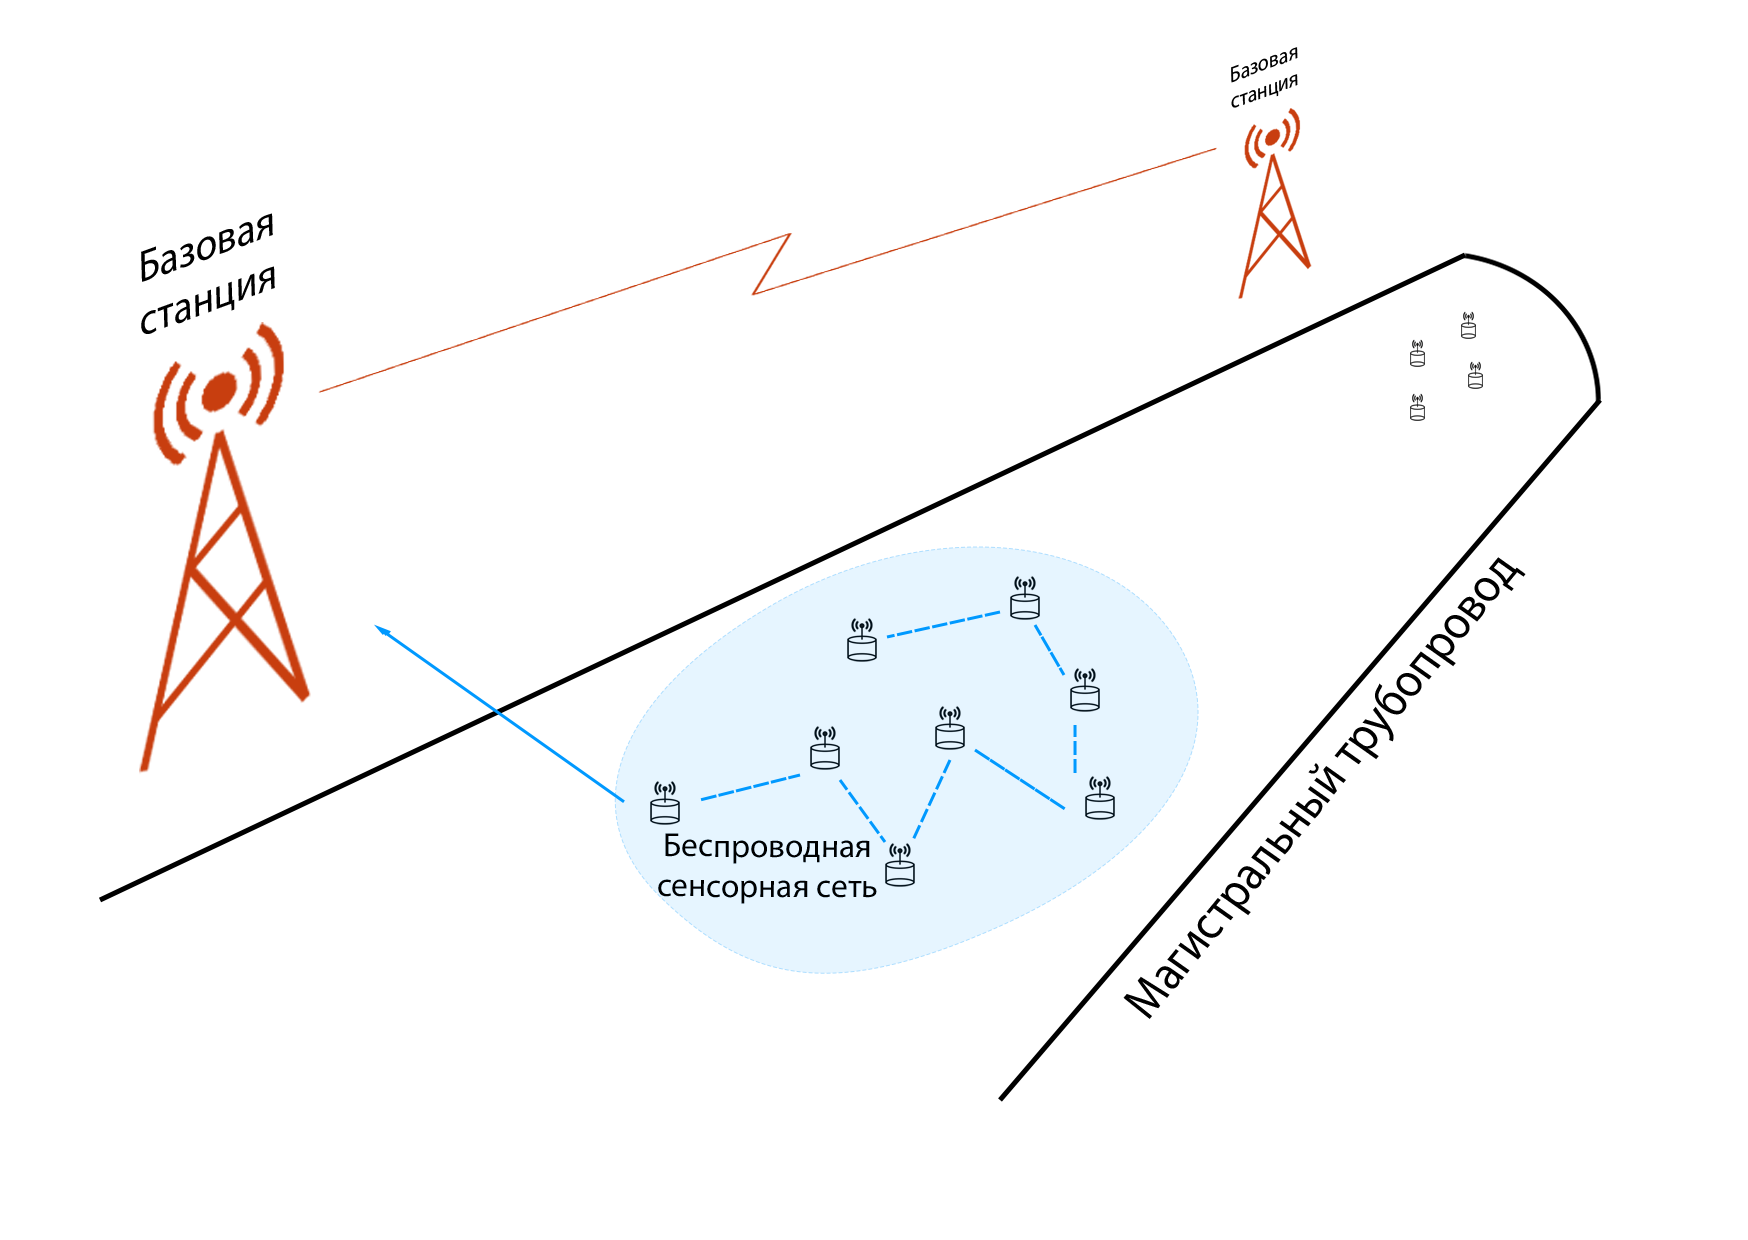
\includegraphics[scale=1.1]{pipeline.png}
%   }
%   \caption{Беспроводная сеть вдоль магистрального трубопровода}\label{fig:part2_pipeline}
% \end{figure}

% В \cite{Anupama2014, Jawhar2007} авторы предлагают иерархическую сенсорную сеть для мониторинга трубопроводов, в которой третий уровень иерархии сети представлен базовыми станциями, покрывающими весь линейный участок.

% Один из современных методов обнаружение утечек и мониторинга в реальном времени является использование беспроводной сети связи на базе стационарных объектов -- базовых станций и  беспилотных летательных аппаратов  (БПЛА, Unmanned Aerial Vehicle, UAV) \cite{Aljuaid2020}. В \cite{Fedorova2020} рассматривается использование БПЛА для мониторинга нефтепроводов. Предлагается математическая модель для определения состава группы БПЛА и метода ее базирования.

Безопасность на месторождении является самой важной задачей любого предприятия. Большинство нефгазовых месторождений в России охватывают огромные площади и находятся на удалении в треднодоступных регионах. Сегодня обеспечение безопасности персонала это задача, которая включает безопасность не только в течение рабочего процесса на технологических объектах, непосредственного, но и в течение всего времени нахождения на промысле. Важными объектами, требующие постоянного контроля являются промысловые автодороги. С учетом большой удаленности технологических объектов на промысле друг от друга для контроля над промысловыми автодорогами целесообразно организовать системы беспроводного видеонаблюдения на дорогах \cite{Vish2015} (Рисунок \ref{fig:part2_roadisdeunit}). Одним из наиболее перспективных решений на транспортных участках является организация автомобильных сетей (Vehicular ad hoc network, VANET) \cite{Massobrio2020, Campolo2015}. Для развертывания таких сетей хорошо подходит БШС. Организации БШС вдоль автодорог посвящено ряд зарубежных и отечественных работ. Большиство работ касаются проблемы размещения придорожных объектов (Roadside Unit, RSU) или другими словами БС вдоль автодорог. В \cite{Cavalcante2012, KHireddine2020} предложены модели, используюящие генетический алгоритм для решения задачи о максимальном покрытии. Максимизация покрытия БШС с учетом ограничения стоимости БС представлена в работах \cite{BenBrahim2014, Vishnevsky2016_optimization}. В работах \cite{Liu2014, Gao2018, Jalooli2019} предложены новый модели размещения БС с учетом характеристик трафика на участках. В \cite{Reis2014} представлена задача размещения БС для протокола IEEE 802.11p/Wave, позволяющая организовать связь для объектов движущихся на скоростях до 200 км/ч.   В \cite{Guerna2021} предложена модель размещения БС с помощью муравьиного алгоритма. В работах \cite{Cavalcante2012, Liu2017} в качестве ограничений учитываются временные ограничения при размещения БС. В \cite{Bao2018} предлагают жадный алгоритм для минимизации RSU c условием ограничения задержек между любыми двумя узлами сети. В работе \cite{Ivanov2018} представлены задача размещения RSU вдоль линейного участка протяженной автомагистрали. 

% \begin{figure}[ht]
%   \centerfloat{
%       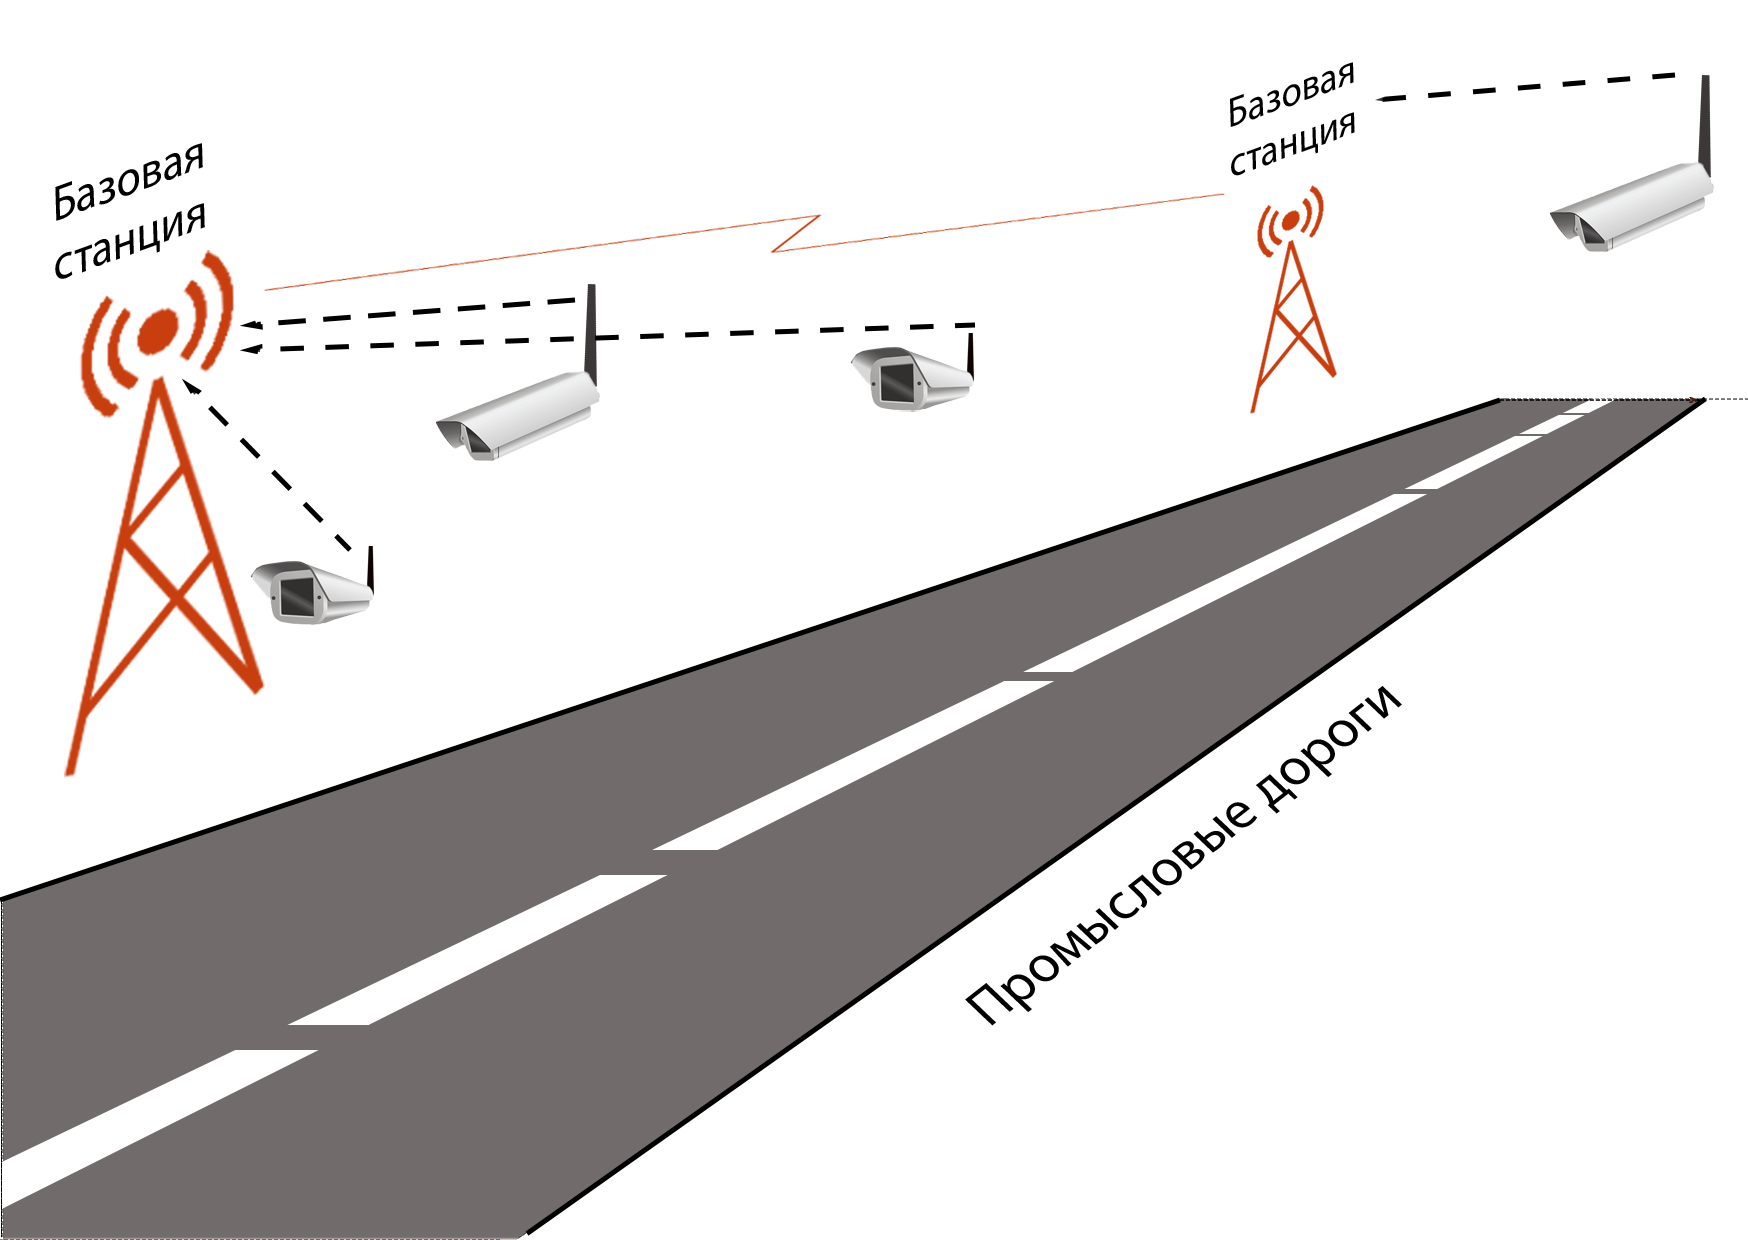
\includegraphics[scale=1.1]{roadsideunit.png}
%   }
%   \caption{Беспроводная сеть вдоль автомобильных дорог}\label{fig:part2_roadisdeunit}
% \end{figure}



% Задача размещения также актуально для беспроводных сетей.

% В работе \cite{Alduraibi2016} предложены модели размещения узлов беспроводной сенсорной сети (WSN, Wirelss Sensor Network), максимизирующий покрытие линейного участка трубопровода. В \cite{Aria2020} авторы представляют во внимание модель размещения узлов WSN обнаружения повреждений на трубопроводе, учитывающие зоны, которые будет контролировать только обслуживания персонал. В работах \cite{Hussein2020, Varshney2018, Varshney2021} представлены модели размещения узлов WSN минимизирующее суммарное энергопотребление. В \cite{Li2020, Albaseer2019} предложен модели кластеризации узлов БШС, в \cite{Albaseer2019} предлагают модели БШС для мониторинга утечек вдоль нефте-- и газопроводов.

% В отличие от большинства реализаций БШС вдоль трубопроводов, где используется одноуровневая реализация сети, в данной диссертации, согласно широко используемой классификации \cite{Jawhar2009, Varshney2015, Abbas2018, Wang2011, Jawhar2013}, будет предложено иерархическая БШС сеть c линейной топологии. Данные с полевых измерительных устройств собираются шлюзом. Именно с этих шлюзов вся информация будет собираться через систему размещенных БС. В случае проектирования БШС для видеонаблюдения, вся поток будет идти на БС непосредственно с антенн камер видеонаблюдения. Для обеспечения масштабируемости сети и быстрое развертывание новых устройств, \fixme{в том числе мобильные обходчики} ставится задача максимального покрытия всего участка.

% Еще одним немаловажным линейным объектом любого промысла, требующим постоянного контроля является сеть промысловых дорог. С учетом большой удаленности друг от друга объектов нефтегазовой отрасли друг от друга целесообразно организовать телекоммуникационную сеть вдоль протяженных автодорог для контроля данного линейного участка с помощью информации с систем видеонаблюдения \cite{Vish2015} (Рисунок \ref{fig:part2_roadisdeunit}). Одним из наиболее перспективных решений на транспортных участках является организация автомобильных сетей (Vehicular ad hoc network, VANET) \cite{Massobrio2020, Campolo2015}. Для решения данной проблемы хорошо подходит БШС. Организации БШС вдоль автодорог посвящено ряд зарубежных и отечественных работ. 








% Размещение БС вдоль линейного участка приобретают все большую актуальность на сегодняшний день. Большиство работ касаются проблемы размещения придорожных объектов (Roadside Unit, RSU) или другими словами БС вдоль автодорог. 

% Задача оптимального размещения БС нашла свое широкое отражениие в исследованиях зарубежных и отечетсвенных авторов. Большиство работ касаются проблемы размещения придорожных объектов (Roadside Unit, RSU) или другими словами БС вдоль автодорог. В \cite{Cavalcante2012} предложена модель, используюящая генетический алгоритм для решения задачи о максимальном покрытии. Максимизация покрытия БШС с учетом ограничения стоимости БС представлена в работах \cite{BenBrahim2014, Vishnevsky2016_optimization}. В работах \cite{Liu2014, Gao2018, Jalooli2019} предложены новый модели размещения БС с учетом характеристик трафика на участках. В \cite{Reis2014} представлена задача размещения БС для протокола IEEE 802.11p/Wave. В \cite{Guerna2021} предложена модель размещения БС с помощью муравьиного алгоритма. В работах \cite{Cavalcante2012, Liu2017} в качестве ограничений учитываются временные ограничения при размещения БС. В \cite{Bao2018} предлагают жадный алгоритм для минимизации RSU c условием ограничения задержек между любыми двумя узлами сети. В работе \cite{Ivanov2018} представлена задача размещения RSU вдоль линейного участка протяженной автомагистрали. 


% Представление задачи размещения БС вдоль автодорог в виде одномерной задачи нашло свое широкое применение \cite{Ivanov2018, Reis2014, Vishnevsky2016_optimization, Liu2014, Gao2018, Jalooli2019, Zhang2017}. В нашем случае является также эффективным для применения вдоль промысловых дорог между удалленными на большие расстояния объектами нефтегазовых отрасли.

% Задача размещения также актуально для беспроводных сетей. В работе \cite{Alduraibi2016} предложены модели размещения узлов беспроводной сенсорной сети (WSN, Wirelss Sensor Network), максимизирующий покрытие линейного участка трубопровода. В \cite{Aria2020} авторы представляют во внимание модель размещения узлов WSN обнаружения повреждений на трубопроводе, учитывающие зоны, которые будет контролировать только обслуживания персонал. В работах \cite{Hussein2020, Varshney2018, Varshney2021} представлены модели размещения узлов WSN минимизирующее суммарное энергопотребление. В \cite{Li2020, Albaseer2019} предложен модели кластеризации узлов БШС, в \cite{Albaseer2019} предлагают модели БШС для мониторинга утечек вдоль нефте-- и газопроводов.

% В отличие от большинства реализаций БШС вдоль трубопроводов, где используется одноуровневая реализация сети, в данной диссертации, согласно широко используемой классификации \cite{Jawhar2009, Varshney2015, Abbas2018, Wang2011, Jawhar2013}, будет предложено иерархическая БШС сеть c линейной топологии. Данные с полевых измерительных устройств собираются шлюзом. Именно с этих шлюзов вся информация будет собираться через систему размещенных БС. В случае проектирования БШС для видеонаблюдения, вся поток будет идти на БС непосредственно с антенн камер видеонаблюдения. Для обеспечения масштабируемости сети и быстрое развертывание новых устройств, \fixme{в том числе мобильные обходчики} ставится задача максимального покрытия всего участка.


\section{Математические модели синтеза топологии сети для охвата линейного участка в виде задачи целочисленного линейного программирования}

В середине прошлого века с появлением первых компьютеров свою широкую популярность приобрела область математики, задачей корой является поиск экстремальных решений на допустимых множествах. Это положило начало математическому программированию. Сегодня одним из наиболее интересных классов задач математического программирования являются задачи ЦЛП. Эти задачи формулируются как задачи линейного программирования (ЛП) с дополнительным ограничением целочисленности переменных. Для задач ЛП существуют эффективный алгоритм решения - симплекс-метод, предложенный Д. Данцигом \cite{Dantzig1963}. Добавление ограничение целочисленности портит свойство выпуклости и полиномиальности задачи ЛП. \fixme{[Ссылка]}. Основная проблема, возникающая при решении практических задач на конечных множествах --  «проклятие размерности» \cite{Pershin2013}. C увеличением размерности пространства количества данных возрастает экспоненциально. Для решения задач целочисленного программирования распространены методы отсечения и комбинаторные методы \cite{Alekseev1987, Sukharev1986}. 

Идея методов отсечения заключается в решении задачи ЛП без учета целочисленности. Если полученное решение оптимальное решение не является целочисленным, то вводятся дополнительные ограничения, отсекающие нецелочисленные вершины многогранника и вновь повторяется процедура поиска. Существующие алгоритмы отсечения отличаются друг от друга способами формирования дополнительных ограничений для отсечения нецелочисленности. Методы отсечения имеют общий существенный недостаток. Практический опыт показал плохую сходимость. Для повышения эффективности вычислительных алгоритмов были предложены комбинаторные методы, основанные на упорядоченном переборе наиболее перспективных вариантов. 


Одним из наиболее популярных комбинаторных методов для решения не только целочисленных, но и частично целочисленных задач ЛП является метод ветвей и границ (МВиГ). Впервые данный метод  был предложен Лэнд и Дойгом в работе \cite{Land1960}. Существуют различные методы типы ветвей и границ. Все они о снованы на последовательном разбиении допустимого множества на подмножества и вычислении оценок, позволяющие отбрасывать подмножества, не содержащие решение задачи.

%  Его суть заключается в упорядоченном переборе вариантов и рассмотрении лишь тех из них, которые оказываются по определенным признакам перспективными, и отбрасывании бесперспективных вариантов. 



% Класс задач ЦЛП обладают замечательным свойством, их решения всегда целые при целых правых частях системы условий \cite{Pershin2013}. Следовательно, задачи такого рода можно решать как задачи линейного программирования, сняв условие целочисленности переменных.

Для  практических задач существуют готовые коммерческие продукты, эффективно решающие задачу оптимизацию общего вида. Можно выделить наиболее популярные из них: MatLab Optimization ToolBox, Gurobi Optimizer, GLPK, CPLEX. Подробный обзор коммерческих, бесплатных и продуктов с открытым исходным кодом для задач линейного программирования представлен в работах \cite{Meindl2012, Ku2016, Anand2017}. 

В данной секции будет представлена математическая модель в виде задачи целочисленного линейного программирования для решения задачи максимизации телекоммуникационного покрытия участка при развертывании базовых станций БШС.

\subsection{Постановка задачи}

Проблема формулируется следующим образом. Для контроля над заданным линейным участком необходимо разместить базовые приемопередающие станции таким образом, чтобы максимизировать покрытие с ограничением на суммарную стоимость размещенных станций. Необходимо, чтобы любая БС в сети могла быть связана со шлюзами на концах участка через систему размещенных станций.

Задано множество станций $S = \{s_j\}$. Каждой станции приписаны параметры  $s_j = \{r_j, \{R_{jq}\}, c_j \}$, $j = \overline{1,m}; q = \overline{1,m}; q \neq j$. 
Каждая БС содержит два модуля радиосвязи - для подключения абонентов и для связи с соседними станциями. Первая характеризуется параметром $r_j$ -- максимальный радиус покрытия станции, вторая характеризуется множеством $\{R_{jq} \}$ -- матрица радиусов связи между $j$-ой и $q$-ой базовыми станциями. Параметр $c_j$ -- это стоимость. 

Задан линейный участок длиной $L$ с концами в точках $a_0$ и $a_{n+1}$. Внутри  отрезка $[a_0, a_{n+1}]$ задано конечное множество точек $A=\{a_i\}, i=\overline{1,n}$; эти точки соответствуют набору свободных мест, где могут быть размещены станции. Каждая точка $a_i$ определяется своей одномерной координатой $l_i$.

Заданы станции специального вида $s_{m+1}$ -- шлюзы. Данные шлюзы размещены на концах $a_0$ и $a_{n+1}$ данного линейного участка. Для данных станций параметр радиуса покрытия $r_{m+1}=0$. Радиус связи и стоимость не заданы.

Требуется разместить станции таким образом, чтобы максимизировать покрытие с условием ограничения на суммарную стоимость $C$.


\subsection{Модель целочисленного линейного программирования}

Перед тем как перейти к постановке задачи оптимизации в виде модели целочисленного линейного программирования, необходимо подготовки параметры БС: радиус связи между станциями $R_{jq}$ и радиус телекоммуникационного покрытия $r_j$ с помощью уравнений расчета дальности связи, представленных в главе 1.



Пусть $y_i^+$ и $y_i^-$, $i= \overline{0,n+1}$ определяют охват покрытия (справа и слева, соответственно) станций, покрывающих точку $a_i$ (Рисунок \cref{fig:part3_station_coverage}). Параметры $y_i^+$ и $y_i^-$ могут принимать только неотрицательные целые значения.

Величины  покрытия для шлюзов $y_0^+, y_0^-, y_{n+1}^+, y_{n+1}^-$ равны 0.

\begin{figure}[ht]
  \centerfloat{
      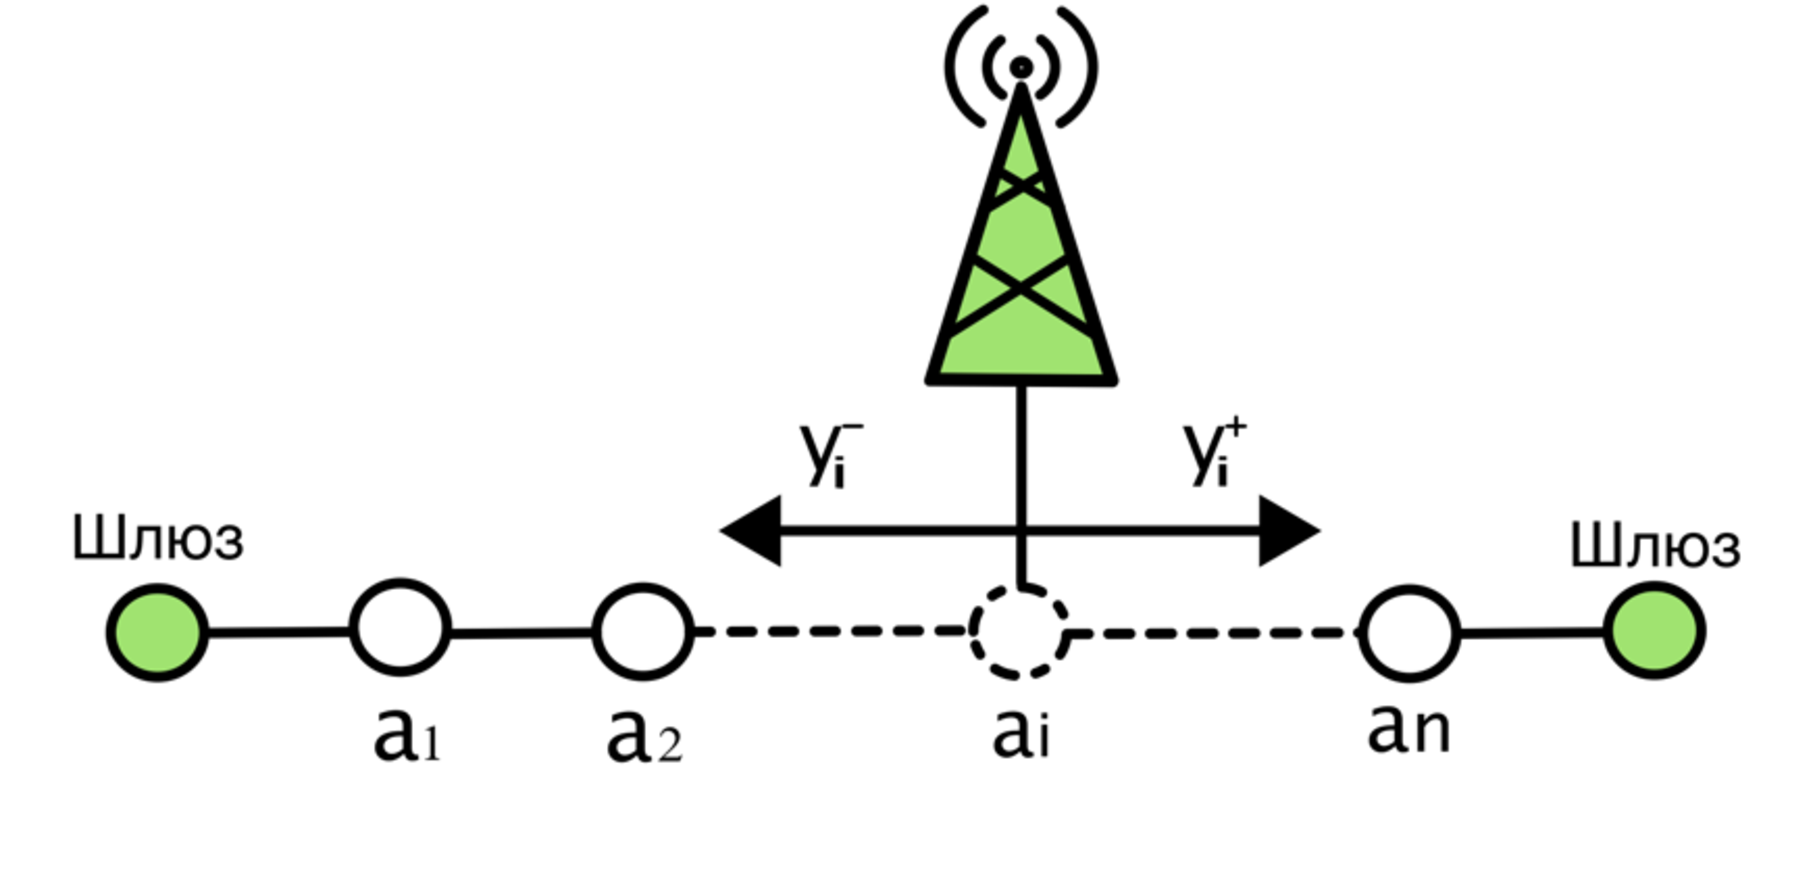
\includegraphics[scale=0.5]{station_coverage.pdf}
  }
  \caption{Охват покрытия станции}\label{fig:part3_station_coverage}
\end{figure}
 
Целевая функция будет представлена как:
\begin{equation}
  \label{eq:part3_objective_function}
  f =  \sum\limits_{i=1}^n (y_i^- + y_i^+) \rightarrow max
\end{equation}

Также введем бинарные переменные $x_{ij}$. Тогда $x_{ij}=1$, если станция $s_j$, размещенная на точке $a_i$, и $x_{ij}=0$ в противном случае; $i= \overline{1, n}$; $j = \overline{1,m}$.

Введем двоичные переменные $ e_i $. Тогда $ e_i = 1 $, если какая-либо станция находится в точке $ a_i $, и $ e_i = 0$  в противном случае; $ i = \overline {1, n} $. Для точек размещения шлюзов $ a_0 $ и $a_{n + 1}$ переменные $ e_0 = 1 $ и $ e_{n + 1} =1 $, соответственно. 

% Let us introduce binary variables $e_i$. Then $e_i$  is equal to 1, if any station is placed at point $a_i$ and $e_i$ is equal to 0 otherwise; $i = \overline{1, n}$. For gateways placement points $e_0$  is equal to 1 and $e_{n+1}$  is equal to 1.

Сформулируем следующую систему ограничений задачи.

По определению \cref{eq:part3_ei}:

\begin{equation}
  \label{eq:part3_ei}
  e_i =  \sum\limits_{j=1}^m x_{ij}, \quad i = \overline{1,n}. 
\end{equation}

Каждая станция должна быть размещена только в одной точке. \cref{eq:part3_xij}:

\begin{equation}
  \label{eq:part3_xij}
  \sum\limits_{i=1}^n x_{ij} \leq 1, \quad j = \overline{1,m}. 
\end{equation}

Значения покрытий не превышают радиус покрытия станции, размещенной в точке $ a_i $, и равны 0, если в точке $a_i$  нет станции \cref{eq:part3_yi_1, eq:part3_yi_2}:


\begin{equation}
  \label{eq:part3_yi_1}
  y_i^+ \leq \sum\limits_{j=1}^m x_{ij} \cdot r_j, \quad i = \overline{1,n};
\end{equation}

\begin{equation}
  \label{eq:part3_yi_2}
  y_i^- \leq \sum\limits_{j=1}^m x_{ij} \cdot r_j, \quad i = \overline{1,n}. 
\end{equation}

Общая область покрытия между любыми двумя точками $ a_i $ и $ a_k $, где расположены станции, не может превышать расстояние между этими точками \cref{eq:part3_yi_3, eq:part3_yi_4}.

\begin{equation}
  \label{eq:part3_yi_3}
  y_i^+ + y_k^- \leq \frac{l_k - l_i}{2} \cdot (e_i + e_k ) + (2 - e_i - e_k ) \cdot L, \quad i = \overline{1,n},  \quad k = \overline{i+1,n+1};
\end{equation}

\begin{equation}
  \label{eq:part3_yi_4}
  y_i^- + y_k^+  \leq \frac{l_i-l_k}{2} \cdot (e_i + e_k) + (2 - e_i - e_k) \cdot L, \quad i = \overline{1,n}, \quad k = \overline{i-1,0},
\end{equation}
где $ l_k $ и $ l_i $ - координаты точек $ a_i $ и $ a_k $, соответственно. Это условие исключает влияние пересечений покрытий станций при вычислении общего значения покрытия между станциями (Рисунок \cref{fig:part3_total_coverage_between_points}).

\begin{figure}[ht]
  \centerfloat{
      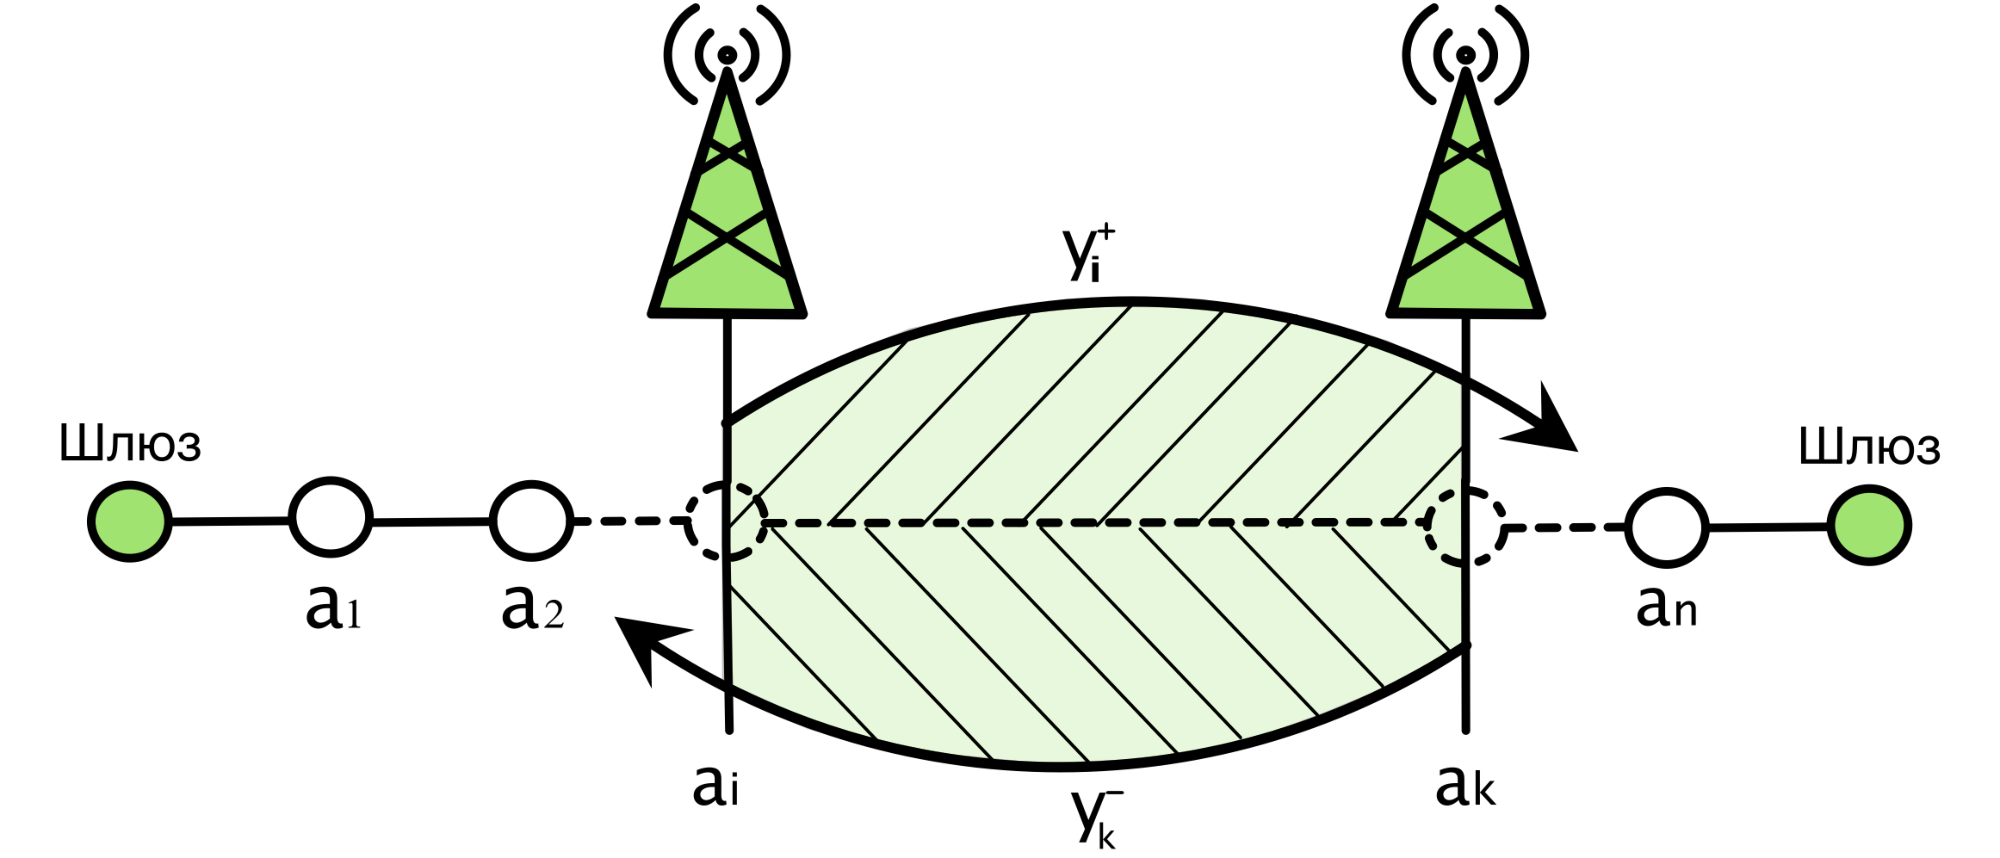
\includegraphics[scale=0.5]{total_coverage_between_points.pdf}
  }
  \caption{Область покрытия между любыми двумя точками}\label{fig:part3_total_coverage_between_points}
\end{figure}

Согласно условиям задачи, станция, расположенная в $ a_i $, должна быть связана хотя бы с одной станцией слева и одной станцией справа, включая станции на конечных точках $ a_0 $ и $a_{n + 1}$. 

Введем бинарные переменные $z_{ijkq}, i = \overline{1,n}; j= \overline{1,m}; k=\overline{1,n},  k \neq i; q= \overline{1,m}, q \neq j$.

Переменная $ z_ {ijkq} = 1$, если в точке $ a_i $ размещена станция $ s_j $ и данная станция связана со станцией $ s_q $, размещенная в точке $ a_k $; и $ z_ {ijkq} = 0 $ в противном случае.

Переменная $ z_{ij0(m + 1)} = 1$, если станция $ s_j $, размещенная в точке $ a_i $, связана со шлюзом $ s_{m + 1} $ в точке $ a_0 $; $ z_{ij0 (m + 1)} = 0 $ в противном случае.
 
Переменная $ z_{ij(n + 1)(m + 1)} = 1 $, если здесь находится станция $ s_j $ в точке $ a_i $ и она связана со шлюзом $ s_{m + 1} $ в точке $ a_{n + 1} $; $ z_{ij0(m + 1)} = 0 $  в противном случае.

Станции должны быть размещены в обеих точках $ a_i $ и $ a_k $, \cref{eq:part3_z_ijkq_1, eq:part3_z_ijkq_2}:

\begin{equation}
  \label{eq:part3_z_ijkq_1}
  z_{ijkq} \leq e_i , \quad i = \overline{1, n}; \quad j = \overline{1, m}; \quad k = \overline{1,n}, k \neq i; \quad q = \overline{1,m}, q \neq j;
\end{equation}


\begin{equation}
  \label{eq:part3_z_ijkq_2}
  z_{ijkq} \leq e_k , \quad k = \overline{1, n}; \quad j = \overline{1, m}; \quad i = \overline{1,n}, i \neq k; \quad q = \overline{1,m}, q \neq j.
\end{equation}

% \fixme{ПЕРЕДЕЛАТЬ  УРАВНЕНИЯ ОГРАНИЧЕНИЯ УСЛОВИЯ СВЯЗИ МЕЖДУ СТАНЦИЯМИ}

% Необходимо, чтобы станция $ s_j $ в точке $ a_i $ была связана с  любой станцией, расположенной в точке $ a_k $, справа от $ a_i $ ($ k> i $) или с правым шлюзом $ s_{m + 1} $ \cref{eq:part3_z_ijkq_3_1, eq:part3_z_ijkq_3_2}. 

% \begin{equation}
%   \label{eq:part3_z_ijkq_3_1}
%   \sum\limits_{k=i+1}^{n} \sum\limits_{\substack{q = 1\\ q \neq j}}^m z_{ijkq} + z_{ij(n+1)(m+1)} = x_{ij} ,  \quad i = \overline{1, n}, \quad j = \overline{1, m}.
% \end{equation}


% Станция $ s_j $, размещенная в $ a_{n} $, справа связана толко со шлюзом $ s_{m + 1} $ на месте $ a_ {n+1}$ \cref{eq:part3_z_ijkq_3_2}. 

% \begin{equation}
%   \label{eq:part3_z_ijkq_3_2}
%   z_{nj(n+1)(m+1)} = x_{nj} \quad j = \overline{1, m}.
% \end{equation}

% Также станция должна быть связана с любой станцией, расположенной в точке $ a_k $ слева от точки $ a_i $ ($ k <i $) или с левым шлюзом $ s_{m + 1} $ \cref{eq:part3_z_ijkq_4_1, eq:part3_z_ijkq_4_2}.

% \begin{equation}
%   \label{eq:part3_z_ijkq_4_1}
%   z_{1j0(m+1)}= x_{ij}, \quad j = \overline{1, m};
% \end{equation}

% Станция $s_j$, размещенная в точке $a_{1}$ слева может быть связана только со шлюзом $s_{m+1}$, расположенном в точке $a_0$ \cref{eq:part3_z_ijkq_4_1}.

% \begin{equation}
%   \label{eq:part3_z_ijkq_4_2}
%   z_{ij0(m+1)} + \sum\limits_{k=1}^{i-1} \sum\limits_{\substack{q = 1\\ q \neq j}} z_{ijkq}= x_{ij}, \quad i = \overline{2, n}, \quad j = \overline{1, m}.
% \end{equation}

% Необходимо, чтобы станция $ s_q $ в точке $ a_k $ была связана с любой станцией справа, расположенной в точке $ a_i $ \cref{eq:part3_z_ijkq_5}.

% \begin{equation}
%   \label{eq:part3_z_ijkq_5}
%   \sum\limits_{i=k+1}^{n} \sum\limits_{\substack{j=1 \\ j \neq q}}^m z_{ijkq} = x_{kq} , \quad k = \overline{1, n-1}, \quad q = \overline{1, m};
% \end{equation}

% Кроме того, станция $ s_q $ в точке $ a_k $ подключена к любой станции слева, расположенной в точке $ a_i $ \cref{eq:part3_z_ijkq_6}. 

% \begin{equation}
%   \label{eq:part3_z_ijkq_6}
%   \sum\limits_{i=1}^{k} \sum\limits_{\substack{j=1 \\ j \neq q}}^m z_{ijkq} = x_{kq} , \quad k = \overline{2, n}, \quad q = \overline{1, m};
% \end{equation}

% Неравенства \cref{eq:part3_z_ijkq_1, eq:part3_z_ijkq_2} и равенства \cref{eq:part3_z_ijkq_3_1, eq:part3_z_ijkq_3_2, eq:part3_z_ijkq_4_1, eq:part3_z_ijkq_4_2, eq:part3_z_ijkq_5, eq:part3_z_ijkq_6} обеспечивают условие симметрии связи между базовыми станциями, расположенными в точках $ a_i $ и $ a_k $, $\forall i, k $ (Рисунок \cref{fig:part3_station_link}).
% \fixme{Скачать, что Zijkq это линк только в одну сторону и необходимо с обепечить связи с двух сторон.}

Стоит отметить, БШС работает в полудуплексном режиме. Переменная $z_{ijkq}$ говорит только о наличии связи для передачи от БС $s_j$ до БС $s_q$. Чтобы обеспечить связь в обоих направлениях, необходимо проверять условия для  $z_{ijkq}$ (от $s_j$ до $s_q$) и для $z_{kqij}$ (от $s_q$ до $s_j$).

Необходимо обеспечить коммуникационную связь справа от БС \cref{eq:part3_z_ijkq_1_1, eq:part3_z_ijkq_1_2}. Станция $ s_j $ в точке $ a_i $ должна быть связана с  любой станцией, расположенной в точке $ a_k $, справа от $ a_i $ ($ k> i $) или с правым шлюзом $ s_{m + 1} $ \cref{eq:part3_z_ijkq_1_1} 

\begin{equation}
  \label{eq:part3_z_ijkq_1_1}
  \sum\limits_{k=i+1}^{n} \sum\limits_{\substack{q = 1\\ q \neq j}}^m z_{ijkq} + z_{ij(n+1)(m+1)} = x_{ij} ,  \quad i = \overline{1, n}, \quad j = \overline{1, m}.
\end{equation}
Требуется чтобы станция, размещенная справа от $s_j$ или правый шлюз $ s_{m + 1} $  были связаны с размещаемой станцией $ s_j $ \cref{eq:part3_z_ijkq_1_2}

\begin{equation}
  \label{eq:part3_z_ijkq_1_2}
  \sum\limits_{k=i+1}^{n} \sum\limits_{\substack{q = 1\\ q \neq j}}^m z_{kqij} + z_{(n+1)(m+1)ij} = x_{ij} ,  \quad i = \overline{1, n}, \quad j = \overline{1, m}.
\end{equation}

Необходимо обеспечить коммуникационную связь слева от БС \cref{eq:part3_z_ijkq_2_1, eq:part3_z_ijkq_2_2}. Станция $ s_j $ в точке $ a_i $ должна быть связана с  любой станцией, расположенной в точке $ a_k $, слева от точки $ a_i $ ($ k <i $) или с левым шлюзом $ s_{0}$ \cref{eq:part3_z_ijkq_2_1} 

\begin{equation}
  \label{eq:part3_z_ijkq_2_1}
  z_{ij0(m+1)} + \sum\limits_{k=1}^{i-1} \sum\limits_{\substack{q = 1\\ q \neq j}}^m z_{ijkq}= x_{ij}, \quad i = \overline{1, n}, \quad j = \overline{1, m}.
\end{equation}
Требуется чтобы станция, размещенная слева от $s_j$ или левый шлюз $ s_{0} $  были связаны с размещаемой станцией $ s_j $ \cref{eq:part3_z_ijkq_2_2}

\begin{equation}
  \label{eq:part3_z_ijkq_2_2}
    z_{0(m+1)ij} +  \sum\limits_{k=1}^{i-1} \sum\limits_{\substack{q = 1 \\ q \neq j}}^m z_{kqij}= x_{ij},  \quad i = \overline{1, n}, \quad j = \overline{1, m}.
\end{equation}


Неравенства \cref{eq:part3_z_ijkq_1, eq:part3_z_ijkq_2} и равенства \cref{eq:part3_z_ijkq_1_1, eq:part3_z_ijkq_1_2, eq:part3_z_ijkq_2_1, eq:part3_z_ijkq_2_2} обеспечивают условие симметрии связи между базовыми станциями, расположенными в точках $ a_i $ и $ a_k $, $\forall i, k $ (Рисунок \cref{fig:part3_station_link}).

\begin{figure}[ht]
  \centerfloat{
      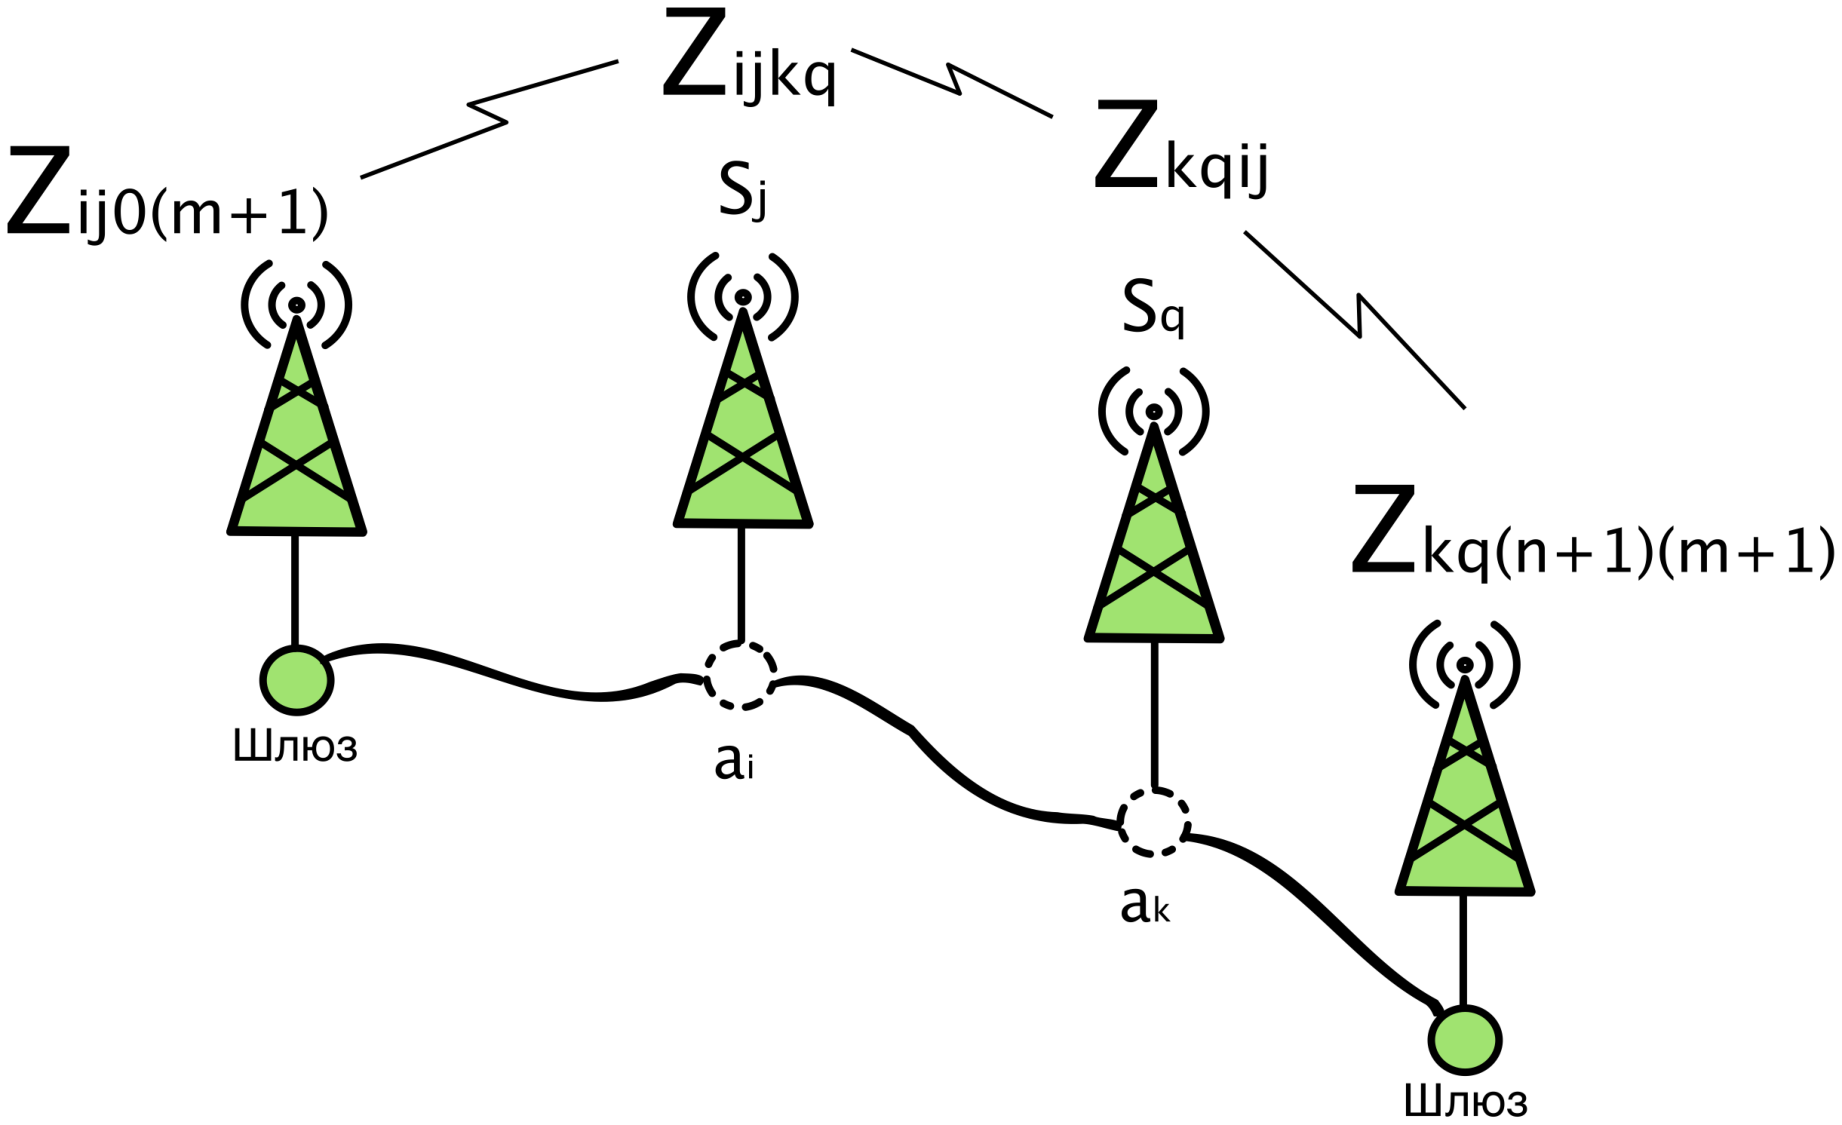
\includegraphics[scale=0.5]{station_link.pdf}
  }
  \caption{Связь между базовыми станциями}\label{fig:part3_station_link}
\end{figure}

Если станции $ s_j $ и $ s_q $ связаны, то максимальный радиус связи размещенных станций должен быть не меньше расстояния между точками $ a_i $ и $ a_k $, где расположены станции $ s_i $ и $ s_q $ (Рис. \cref{fig:part3_station_link_between_points}). Формально это можно записать как \cref{eq:part3_z_ijkq_3, eq:part3_z_ijkq_4}.

 $\forall i= \overline{1,n}$:
\begin{equation}
  \label{eq:part3_z_ijkq_3}
  z_{ijkq}(R_{jq}-(a_i-a_k ))\geq 0, \quad k=\overline{0,i-1}; \quad j=\overline{1,m}; \quad q= \overline{1,m}, q \neq j; 
\end{equation}

\begin{equation}
  \label{eq:part3_z_ijkq_4}
  z_{ijkq} (R_{jq}-(a_k-a_i )) \geq 0, \quad k=\overline{i+1,n+1}; \quad j=\overline{1,m}; \quad q= \overline{1,m}, q \neq j.
\end{equation}

\begin{figure}[ht]
  \centerfloat{
      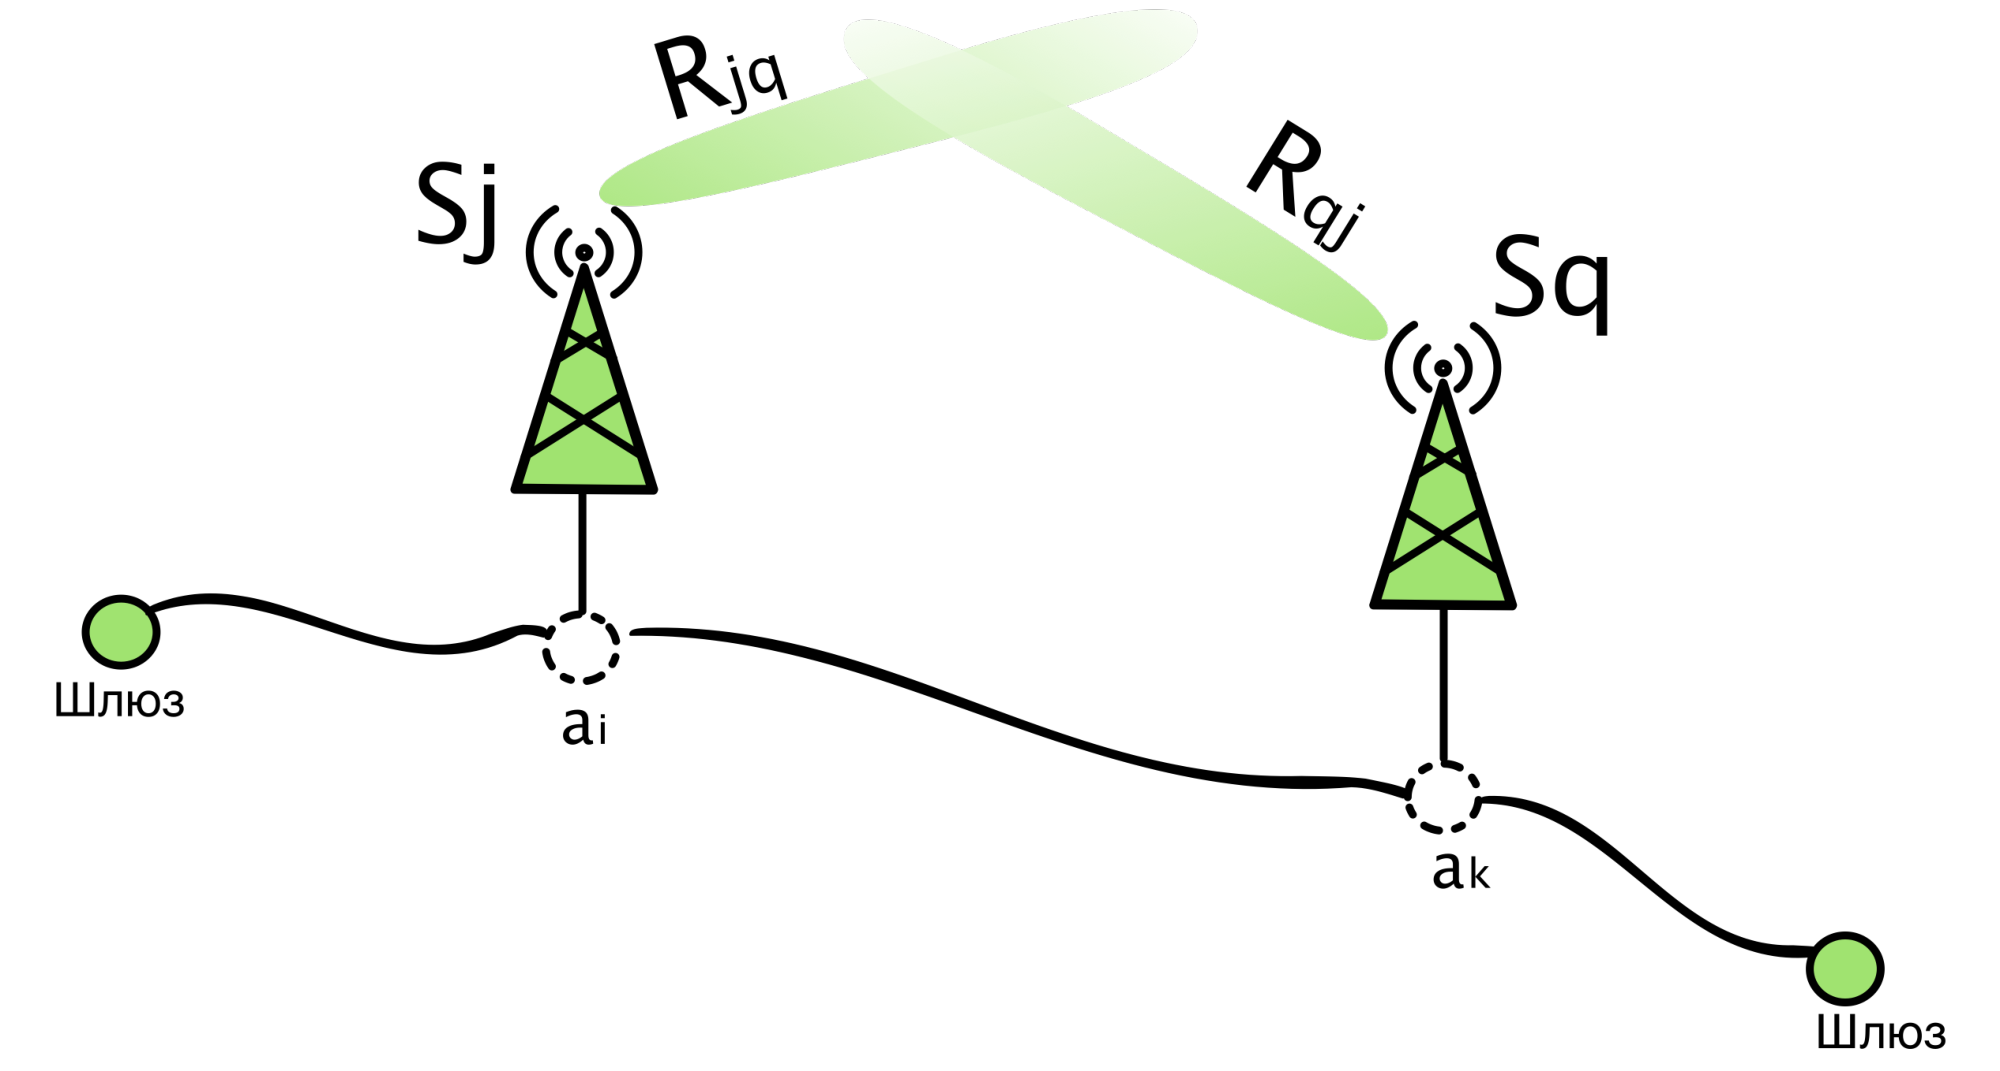
\includegraphics[scale=0.5]{station_link_between_points.pdf}
  }
  \caption{Обеспечение связи с соседней станцией}\label{fig:part3_station_link_between_points}
\end{figure}

Стоимость размещения должна удовлетворять бюджетному ограничению $C$:

\begin{equation}
  \label{eq:part3_cost}
  \sum\limits_{i=1}^n \sum\limits_{j=1}^m x_{ij} \cdot c_j \leq C.
\end{equation}

Работа \cite{Ivanov2018} содержит доказательство NP-трудности для частного случая задачи ЦЛП, когда вдоль линейной территории размещают множество однотипных станций с одинаковыми параметрами. Задача называется NP-трудной, если ей соответсвующая задача распознавания NP-полна \cite{Pershin2013}.  Представленная в данном исследовании модель \cref{eq:part3_objective_function} -- \cref{eq:part3_cost} рассматривает общий случай размещения, когда вдоль линейного участка размещают множество различных станций с разными техническими параметрами. Следовательно, данная задача является также NP-трудной.

Математическая модель рассчитывалась в пакете Optimization Toolbox MATLAB. Числовой пример решения полученной матемаческой модели задачи ЦЛП представлен в приложении \cref{app:ilp_solution}. В приложении также представлена методика расчета дальности связи для обеспечения коммуникации между базовыми станциями и охвата зоны покрытия.


\section{Математические модели синтеза топологии сети для охвата линейного участка в виде экстремальной задачи в комбинаторной форме}

В данной главе была уже представлена математическая модель задачи размещения базовых станций в виде задачи ЦЛП. К сожалению, модели в общем виде не учитывают специфику конкретной задачи. В большинстве практических случаях, поиск решения получается не самым быстрым. Еще одной сложностью при решении задачи в виде ЦЛП является случаи, когда невозможно представить ограничения задачи в линейном виде. 

При проектировании телекоммуникационных сетей важным этапом является оценка характеристик производительности сетей. Такие оценки необходимо учитывать при решении задачи синтеза топологии. Одной из таких характеристик является межконцевая задержка сети. Данную характеристику при наличии кросс-трафика в сети, т.е. с поступлением пакетов на все узлы сети, невозможно представить в линейном виде для модели ЦЛП. Для того чтобы учесть специфику размещения базовых станций БШС и использовать характеристику производительности сети в качестве ограничения задачи, в работе будет представлена задача размещения базовых станций в виде комбинаторной модели в экстремальной форме. Будет предложен алгоритм типа ветвей и границ для решения комбинаторной задачи телекоммуникационного покрытия заданного участка.

Алгоритм на основе метода ветвей и границ основан на следующих построениях, позволяющих уменьшить время перебора:

\begin{enumerate}
  \item Ветвление. Разбиение исходного множества на попарно не пересекающие дочерние подмножества в ходе поиска оптимального решения.
  \item Получение нижних границ. Исследования текущей вершины на возможность закрытия.
\end{enumerate}

Особенность задачи дискретного программирования состоит в том, что они имеют переборный характер. Основная идея комбинаторных алгоритмов -- выделить из множества допустимых решений подмножества, не содержащие оптимальных решений \cite{SigalBook}, для сокращения времени перебора всех возможных вариантов. 




\subsection{Постановка задачи}

Пусть задано множество станций $S=\{s_j\}$ с параметрами $s_j=\{r_j,\{R_{jq} \},p_j, c_j \},j=1,...,m;q=1,...,m;j \neq q $. Каждой БС приписаны параметры $r_j$ -- максимальный радиус покрытия станции, $\{R_{jq} \}$ -- матрица радиусов связи между $j$-ой и $q$-ой базовыми станциями. Также заданы параметры: $p_j$ -- пропускная способность БС и $c_j$ -- стоимость.


Задан отрезок $\alpha$ длины $L$ с концами в точках $a_0$ и $a_{n+1}$. Внутри отрезка $\alpha = [a_0, a_{n+1}]$ задано множество возможных точек размещения станций $A=\{a_i \},i=1,...,n$ с координатами $l_i$. Точка $a_0$ имеет координату $l_0=0$, точка $a_{n+1}$ имеет координату $l_{n+1}=L$. На концах отрезка в вершинах $a_0$ и $a_{n+1}$ стоят станции специального вида -- шлюзы $s_0$ и $s_{m+1}$, соответственно, для которых радиусы покрытия, пропускные способности и стоимости не задаются. Радиусы связи для обеспечения соединения с размещаемыми БС задаются как $R_{0j}$ и $R_{(m+1)j}$, соответственно.
Требуется разместить станции таким образом, чтобы максимизировать область покрытия отрезка $L$ при выполнении требования на наличия связи каждой станции со станциями на концах отрезка (шлюзами) через систему размещенных станций, а также выполнении ограничений на величину времени межконцевой задержки $T$ и суммарную стоимость размещения $C$.


\subsubsection{Формулировка в виде экстремальной задачи на конечном множестве}

\textbf{Допустимой расстановкой} станций назовем такой возрастающий по величине координат $l_i$  набор пар $P = \{a_i, s_j\}, \, a_i \in A,i \neq 0,i \neq n+1;s_j \in S$, для которого выполняются \textbf{требования}:

\begin{enumerate}
  \item  Для каждой пары $(a_i,s_j)$:
      \begin{enumerate}
          \item слева: либо найдется такая пара $(a_k,s_q)$, что, $l_i - l_k \leqslant R_{jq}$  и $l_i - l_k  \leqslant R_{qj}$, либо $l_i-l_0 \leqslant R_{j0}$ и $l_i - l_0 \leqslant R_{0j}$;
          \item справа: либо найдется такая пара $(a_t,s_g)$, что, $l_t-l_i \leqslant R_{jg}$ и $l_t - l_i \leqslant R_{gj}$, либо $l_{n+1}-l_i \leqslant R_{j(m+1)}$ и $l_{n+1}-l_i \leqslant R_{(m+1)j}$. 
\end{enumerate}
Данное требование гарантирует, что любая станция может быть связана со станциями на концах отрезка либо через промежуточные станции, либо непосредственно.
  \item Сумма задержек по всем размещенным станциям меньше заданной величины $T$ – средней межконцевой задержки по времени по всей системе станций:
  \begin{displaymath}
      \label{eq:part3_e2e_delay}
      \sum\limits_{j \in S_\sigma} \overline{T_j} \leqslant T,
  \end{displaymath}
где $S_\sigma$ – множество размещенных станций, $\overline{T_j}$ -- среднее время задержки на станции. Расчет времени задержки с помощью модели массового обслуживания описан в параграфе \cref{part4_e2e_delay_section}.
  \item Суммарная стоимость размещенных станций меньше заданного бюджетного ограничения  $C$.
\end{enumerate}


Каждой допустимой расстановке станций $P$ соответствует величина покрытия $z(P)$, определяемая как суммарная длина всех таких участков $\tau,\tau \subset \alpha$, что каждая точка этих 
участков попадает в зону покрытия, по крайней мере, одной станции, входящих в набор пар $P$.

В дальнейшем для удобства описания алгоритмов введем понятие <<недопокрытия>> отрезка $\alpha$:

\begin{displaymath}
    f(P) = L - z(P)
\end{displaymath}

<<Недопокрытие>> -- это суммарная область заданного участка $L$, которая не охвачена телекоммуникационным покрытиtv БШС. Численно равна разности между суммарным покрытием размещенных базовых станций и длиной всего участка $L$.


Пусть $G$ -- множество всех допустимых расстановок $P$.
Тогда можно сформулировать задачу в виде экстремальной задачи на конечном множестве. 

\underline{\textit{\textbf{Задача 1.}}}

Требуется найти такую допустимую расстановку  $P^*$, что
\begin{equation}
    \label{eq:part3_P}
    P^* = \argmin \limits_{P \in G} f(P)
\end{equation}

Обозначим через $\Gamma$ все множество вариантов размещения станций, необязательно допустимых, из множества $S$ на заданном множестве $A$ возможных точек их размещения.

\subsection{Дерево ветвлений для перебора элементов в множестве \texorpdfstring{$\Gamma$}{Lg}}

Опишем процедуру построения бинарного дерева поиска (дерева ветвлений) для полного перебора без повторений всех элементов множества $\Gamma$. Данная процедура будет использована при построении дерева поиска в алгоритме МВиГ решения \textbf{задачи 1}.

Предполагается, что в множестве $S$ станции упорядочены по не убыванию радиусов покрытия. Описываемая процедура использует известный прием разбиения множества $G$ на подмножества с использованием некоторого параметра. Процесс формирования и последовательность исследования подмножеств обычно представляется с помощью дерева поиска, представляющего собой ориентированное от корня «дерева ветвлений», где каждому подмножеству соответствует вершина на дереве. Множеству $\Gamma$ соответствует корневая вершина. 

\subsubsection{Процесс разбиения исходного множества на дочерние подмножества}

Выбор способа ветвления дерева связан со спецификой задачи. В случае \textbf{задачи 1} спецификой является размещение множества станций $S$ на множестве возможных точках размещения $A$. На каждом узле дерева будем применять дихотомическое ветвление.

\textit{\textbf{Процедура 1.}} Пусть $G_0$, где нижний индекс – номер итерации, исходное множество $\Gamma$. На каждой итерации, начиная с итерации $\nu=0$, текущее подмножество $G_\nu$ разбивается на два подмножества $G^1_\nu$ и $G^2_\nu$. Множество $G_\nu$ обычно называется <<материнским>>, а множества $G^1_\nu$  и $G^2_\nu$  - << потомками>> множества $G_\nu$ или <<дочерними>> множествами (Рисунок \cref{fig:part2_bst_child_nodes}.)

\begin{figure}[ht]
  \centerfloat{
      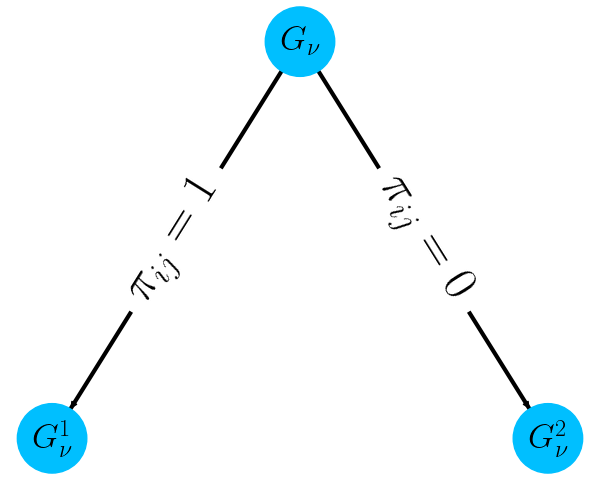
\includegraphics[scale=0.5]{bst_child_nodes.png}
  }
  \caption{Ветвление бинарного дерева}\label{fig:part2_bst_child_nodes}
\end{figure}

В качестве параметра разбиения используется переменная $\pi_{ij}$, принимающей два значения 0 и 1:

\begin{itemize}
    \item $\pi_{ij}=1$, если наложено условие, что на месте $a_i$ может быть расположена БС $s_j$;
    \item $\pi_{ij} = 0$, если наложено условие, что на месте $a_i$ БС $s_j$  располагаться не будет.
\end{itemize}

На каждой  $\nu$-ой итерации в процессе ветвления для множества $G^1_\nu$ задано условие $\pi_{ij}=1$, а для множества $G^2_\nu$  задано условие $\pi_{ij} = 0$.

Все дочерние множества удовлетворяют следующим условиям:

\begin{equation}
    \label{eq:part4_G_cup}
    G^1_\nu \cup G^2_\nu = G_\nu;
\end{equation}


\begin{equation}
    \label{eq:part4_G_cap}
    G^1_\nu \cap G^2_\nu = \varnothing.
\end{equation}

\paragraph{Выбор переменной для разбиения на $\nu$-ой итерации.}

На этапе разбиения любого множества $G_\nu$ все множество переменных $\Pi = \{\pi_{ij}\}$ можно разделить на три подмножества: 

\begin{itemize}
  \item $\Pi^+$ -- «фиксированные» переменные, для которых $\pi_{ij}=1$;
  \item $\Pi^-$ -- «запрещенные» переменные, для которых $\pi_{ij}=0$;
  \item $\Pi^f$ -- «свободные» переменные, для которых значения на данной итерации еще не заданы.
\end{itemize}
Правило выбора переменной для разбиения множества $G_\nu$. Для разбиения множества $G_\nu$ на каждой итерации выбирается переменная из множества $\Pi^f$ c наименьшим индексом $j$ среди всех переменных с наименьшим индексом $i$. Таким образом, сначала определяется незанятое место размещения $a_i$ с наименьшим номером (индексом $i$) и на нем размещается еще не размещенная станция $s_j$ с наименьшим номером (индексом $j$).

\subsubsection{Движение по дереву ветвлений.}

После разбиения очередного подмножества $G_\nu$ на два подмножества $G^1_\nu$  и $G^2_\nu$, последним на дереве ветвлений присваиваются порядковые индексы $G_{\nu+1}$ и $G_{\nu+2}$, соответственно (Рисунок \ref{fig:part2_tree_traversal}).
При формировании дерева ветвлений различаются два типа шагов: «прямой» и «обратный». Прямой шаг -- это движение «в глубину» по той же ветви дерева, реализующее очередное разбиение множества $G_\nu$ на два потомка, и обратный шаг, реализующий переход от множества $G_\nu$  к одному из ранее сформированных подмножеств. Обратный шаг делается в том случае, когда: либо получено множество $G_\nu$, состоящее из единственного элемента, либо множество $G_\nu$  при данном наборе значений переменных $\pi_{ij}$, выделяющих данное подмножество $G_\nu$ из множества $G_0$, пусто. В этих случаях соответствующая вершина дерева называется «закрытой».

\begin{figure}[ht]
  \centerfloat{
      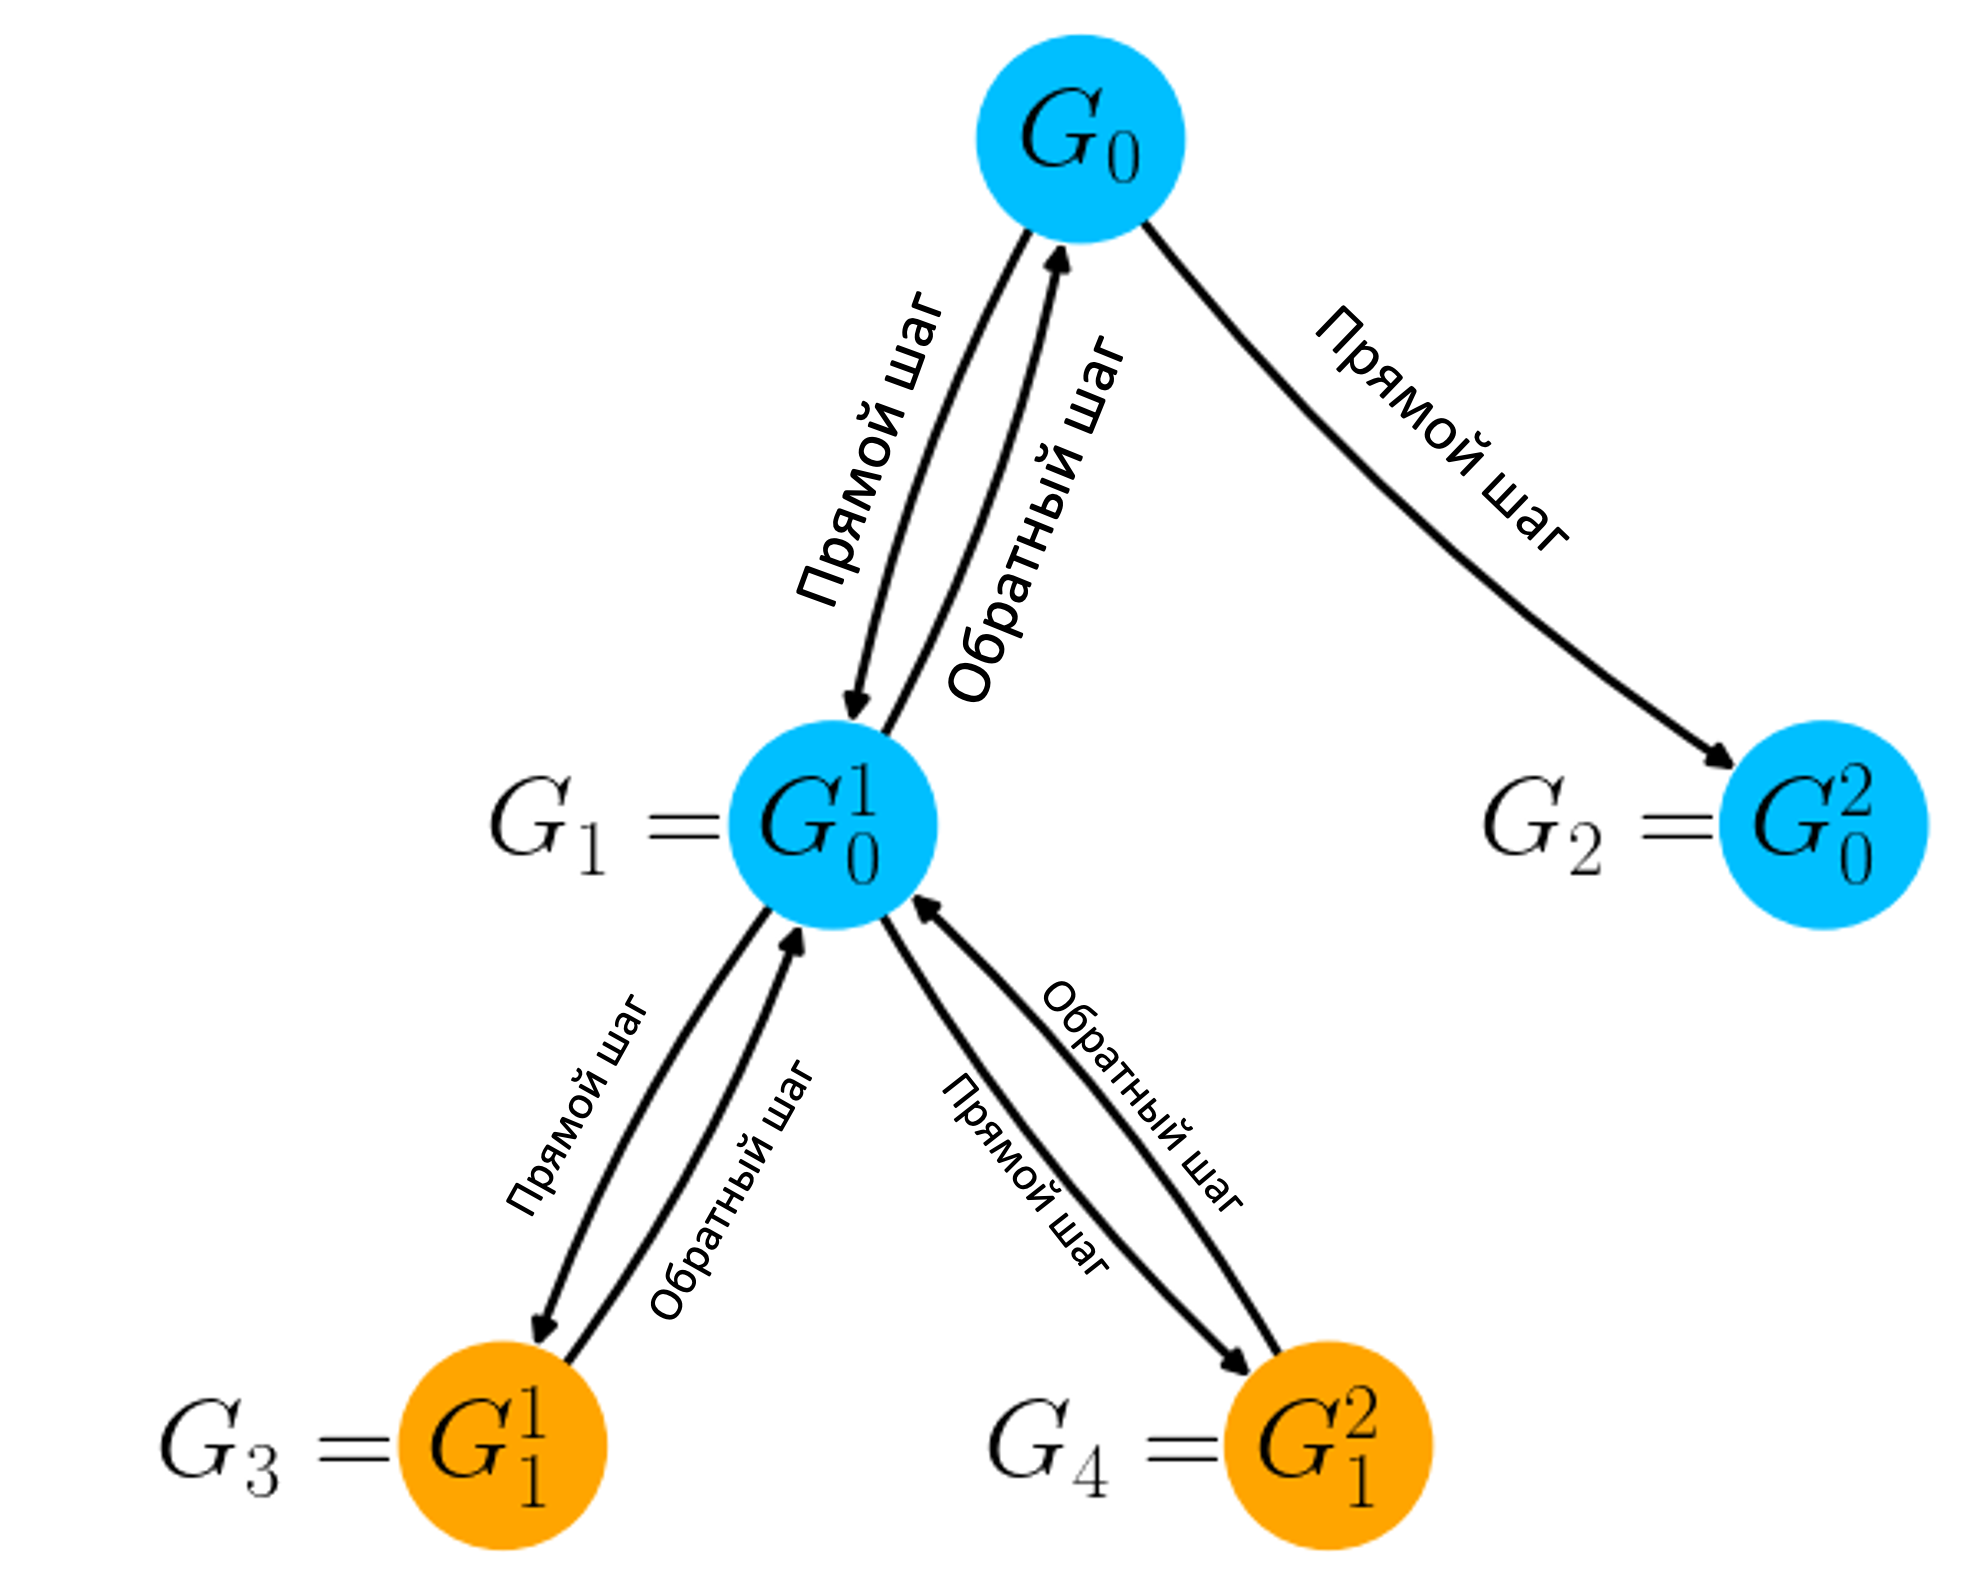
\includegraphics[scale=0.8]{tree_traversal.png}
  }
  \caption{Движение по дереву поиска}\label{fig:part2_tree_traversal}
\end{figure}

Для движения по дереву будем использовать правило \fixme{LIFO}. На основании этого правила прямые шаги будут выполняться до тех пор, пока не будет получена закрытая вершина. На дереве ветвлений это соответствует продолжению движения по той же ветви дерева. При этом из двух множеств $G^1_\nu$  и $G^2_\nu$ первым будет исследоваться на возможность закрытия соответствующей вершины множество $G^1_\nu$ (левый дочерний узел дерева). Если вершина не будет закрыта, то из неё будет продолжено дальнейшее движение по той же ветви -- выполнение прямого шага. Если вершина будет закрыта, то выполняется обратный шаг: для продолжения движения будет выбрана незакрытая вершина с наибольшим порядковым номером $\nu$ среди всех висячих вершин дерева (последняя сформированная вершина из нерассмотренных). Процедура будет завершена, когда все вершины дерева будут закрыты.

Выполнение условия \cref{eq:part4_G_cup, eq:part4_G_cap} гарантирует, что в результате завершения работы \textit{\textbf{процедуры 1}} будут просмотрены все элементы множества $\Gamma$ без повторений. Эти же условия определяют фундаментальное свойство дерева ветвлений: на каждой итерации объединение множеств $G_\nu$ всех висячих вершин дерева дает исходное множество $G_0$ корневой вершины.

\subsection{Метод ветвей и границ для задачи размещения БС} \label{BnB}
Для построения алгоритма типа ветвей и границ для решения \textbf{задачи 1} с использованием \textit{\textbf{процедуры 1}} достаточно разработать методы исследования вершин дерева на возможность их закрытия.

В соответствии с техникой МВиГ закрытие вершины в результате исследования, соответствующего ей множества $G_\nu$ возможно в трех случаях.

\underline{\textit{\textbf{Случай 1.}}} Множество $G_\nu$ -- пусто, т.е. доказано, что в множестве $G_\nu$ при данном наборе фиксированных и запрещенных переменных $\pi_{ij}$ нет ни одной допустимой расстановки $P$.

\underline{\textit{\textbf{Случай 2.}}} Доказано, что в множестве $G_\nu$ не может быть допустимой расстановки P с меньшим значением целевой функции \cref{eq:part3_P}, чем у лучшей расстановки $\widehat{P}$ из уже найденных. Значение функции $f(\widehat{P})$ называется «рекордом», а расстановка $\widehat{P}$ -- «рекордным решением». В качестве начального рекорда принимается число заведомо большее искомого оптимального решения, например,  длина всего отрезка $L$.

\underline{\textit{\textbf{Случай 3.}}} Найдено оптимальное решение \textbf{задачи 1} на множестве $G_\nu$.
Прежде, чем рассмотреть эти три случая, запишем важное свойство любого множества $G_\nu$, являющееся следствием принятого правила выбора свободной переменной для разбиения очередного множества $G_\nu$ при прямом шаге. 



\subsubsection{Исследование случаев 1 – 3}

\textit{\textbf{Свойство 1.}} Пусть для исследуемого множества $G_\nu, \nu > 0$, точка $a_k$ -- любое из мест, на которых уже размещена станция из множества $S$ в соответствии с набором фиксированных и запрещенных переменных $\pi_{ij}$, выделяющим данное множество из множества $G_0$. Тогда для всех мест «слева» от $a_k$, т.е. точек $a_i$, $i<k$, размещение станций уже определенно. В ходе движения по дереву ветвлений на точках  либо были размещены станции при условии $\pi_{ij} =1 , \forall i, j$, либо эти точки $a_i$ остались пустыми при условии $\pi_{ij} =0 , \forall i, j$.

\underline{\textit{\textbf{Случай 1.}}}

Проверка текущего множества $G_\nu$ на пустоту состоит в установлении факта невозможности выполнения \textbf{требования 1 -- 3}, введенных ранее при определении допустимой расстановки.




\paragraph{Проверка выполнения условия связи между размещенными БС}

Построим алгоритм проверки выполнения \textbf{требования 1}.
% \fixme{Рассмотрим сначала исходное множество  $G_0 = \Gamma$. Необходимое условие выполнения требования 1: расстояния от точки $a_0$ до точки $a_1$ и от точки $a_n$  до точки $a_{n+1}$ должны быть не больше максимального радиуса связи между станциtq из множества $S$ и шлюзом, и расстояние между двумя любыми смежными точками $a_i, i=1,...n$, должно быть не больше чем радиус связи из оставшихся БС в множества $S$. сли в результате проверки оказывается, что эти условия не выполняются, то множество $G_0$ допустимых расстановок пусто и \textbf{Задача 1} не имеет решения.}


% Необходимое условие выполнения требования 1: расстояние между двумя любыми смежными точками $a_i, i=1,...n$, должно быть не больше, чем второй по величине после максимального радиус связи у заданного множества, а расстояния от точки $a_0$ до точки $a_1$ и от точки $a_n$  до точки $a_{n+1}$ должны быть не больше максимального радиуса связи среди радиусов связей станций множества $S$. Если в результате проверки оказывается, что эти условия не выполняются, то множество $G_0$ допустимых расстановок пусто и \textbf{Задача 1} не имеет решения.

Рассмотрим проверку для  множества  $G_\nu, \nu>0$. Пусть множество $G_\nu$  образовано разбиением материнского множества при помощи переменной $\pi_{kt}=1$, и множество содержит более одного распределения $P$.
Алгоритм проверки состоит из \textbf{3 шагов}.

\textbf{Шаг 1}. Проверяем, что каждый из радиусов $R_{th}$ и $R_{ht}$, где $h$ – индекс станции, размещенной на ближайшей к точке $a_k$ слева точке $a_d$, больше расстояния $l_k-l_d$. 

\textbf{Шаг 2}. Проверяем, что как радиус $R_{tj}$, так и максимальный радиус $R_{jt}$ среди еще нераспределенных станций не меньше расстояния между точкой $a_k$ и ближайшей к ней точкой справа $a_i$.  Если все станции распределены, то множество $G_\nu$ состоит из единственного варианта распределения и этот случай будет рассмотрен далее.

\textbf{Шаг 3}. Проверяем, что, если количество нераспределенных станций больше 1, то расстояние между двумя любыми смежными точками $a_i, i=k+1,...,n$, не больше, чем второй по величине после максимального радиус связи у еще не распределенного множества станций, а расстояние между точками $a_{n+1}$ и $a_n$  не больше, чем максимальный радиус связи среди нераспределенных станций. Если осталась только одна нераспределенная станция, то проверяем, что среди еще незанятых точек справа от точки $a_k$  есть, по–крайней мере, одна такая точка, что расстояния от этой точки до точки $a_k$ и одновременно от этой точки до точки $a_{n+1}$ не больше, чем  радиус связи у нераспределенной станции.

Если в результате проверки оказывается, что, хотя бы на одном из шагов получен отрицательный результат, то множество $G_\nu$ -- пусто, соответствующая этому множеству на дереве поиска вершина должна быть закрыта и далее выполняется шаг обратного хода в соответствии с \textbf{Процедурой 1}.

Если множество $G_\nu$ образованно разбиением материнского множества при помощи переменной $\pi_{kt}=0$ и $a_v$ -- точка с наибольшим индексом, среди точек, на которых уже размещены станции (с учетом точки $a_0$ ), то надо проверить, что расстояние между точками $a_v$ и $a_k$ не больше, чем максимальный радиус среди радиусов связи у еще нераспределенных станций. Если проверка отрицательна, то множество $G_\nu$  - пусто, соответствующая этому множеству на дереве поиска вершина должна быть закрыта и выполняется шаг обратного хода в соответствии с \textbf{Процедурой 1}.

Проверка \textbf{требований 2 и 3} сводится к установлению факта не превышения суммарных величин стоимости и межконцевой задержки заданным ограничениям.

\underline{\textit{\textbf{Случай 2.}}}
Построим оценку величины «недопокрытия» для множества $G_\nu$, полученного из материнского множества добавлением условия $\pi_{kt}=1$. Частичным «недопокрытием» назовем величину $\Delta(k,d,p,t)$, которая вычисляется по формуле:

\begin{equation}\label{eq:part4_delta}
\Delta(k,d,p,t) = max\{\left(a_{k} - a_{d} \right) - \left(r_{p} + r_{t} \right), 0\}.
\end{equation}

Частичное «недопокрытие» \cref{eq:part4_delta} определяется для любых двух точек $a_d$ и $a_k$ ($k>d$), на которых расположены станции $s_p$ и $s_t$ при условии, что между этими точками нет других станций. Для любой расстановки $P$ «недопокрытие» $f(P)$ вычисляется как сумма всех «недопокрытий» $\Delta(k,d,p,t)$ между местами размещения станций, включая концы отрезка $\alpha$, на которых стоят станции особого типа $s_0$ и $s_{m+1}$.

Построим нижнюю оценку $W(G_{\nu} )$ для недопокрытий $f(P)$ расстановок $P$ множества $G_\nu$, т.е. 

\begin{displaymath}
W(G_\nu) \leq f(P), P \in G_\nu. 
\end{displaymath}

Если $W(G_\nu) \geq f(\widehat{P})$, то множество $G_\nu$ не может содержать расстановки, лучше уже найденной расстановки $\widehat{P}$, тогда соответствующая множеству $G_\nu$  вершина на дереве поиска должна быть закрыта и далее выполняется шаг обратного хода в соответствии с  \textit{\textbf{процедурой 1}}. 

Построим оценку «недопокрытия» для множества $G_\nu$, полученного из материнского множества добавлением условия $\pi_{kt}=1$. Оценку будем искать в виде суммы

\begin{equation}\label{eq:part2_noncoverage_estimation}
  W\left(G_\nu\right) = w_1 \left(G_\nu \right) + w_2 \left(G_\nu \right). 
\end{equation}

Величина $w_1 \left(G_\nu \right)$ вычисляется как сумма все частичных «недопокрытий» слева от вершины $a_k$ и величины радиуса покрытия размещаемой станции $r_t$. Оценку $w_2 \left(G_\nu \right)$ вычислим «для недопокрытия» справа на части $\beta$ до конца отрезка $\alpha$ (точки $a_{n+1}$). Данную оценку получим релаксацией условий, определяющих допустимую расстановку станций на участке $\beta$. Найдем такое подмножество $S_\beta$ множества станций $S$, состоящее из еще не размещенных станций и дающее минимальное «недопокрытие» на участке $\beta$ при выполнении только условий 2) – 4). Для этого сформулируем следующую задачу булевого программирования. Введем булеву переменную $x_j$. Тогда $x_j = 1$, если станция $s_j$ будет размещена, $x_j = 0$ -- в противном случае.

\underline{\textit{\textbf{Задача 2.}}}
\begin{displaymath}
    z = |\beta| - \sum\limits_{x_j \in S_\beta} 2r_j x_j \rightarrow min.
\end{displaymath}
при условии:

\begin{equation}\label{eq:part4_task2_cost}
    \sum\limits_{x_j \in S_\beta} c_j x_j \leqslant C,
\end{equation}

\begin{equation}\label{eq:part4_task2_m}
    \sum\limits_{x_j \in S_\beta} x_j \leqslant m,
\end{equation}

\begin{displaymath}
    x_j \in \{0, 1\},
\end{displaymath}
где $|\beta|$ -- длина отрезка $\beta$, $m$ -- число свободных мест для размещения станций на отрезке $\beta$, $r_j$ -- радиуc покрытия станции $s_j$, $c_j$ - стоимость станции $s_j$ и $C$ -- бюджетное ограничение.

Эффективность использования оценки в методе ветвей и границ определяется точностью оценки и временем ее вычисления. \underline{\textit{\textbf{Задача 2}}} -- это задача ЦЛП, являющаяся трудно решаемой \cite{Gari}. На основании \underline{\textit{\textbf{задачи 2}}} можно получить две оценки менее точные, но имеющие более эффективные методы решения. Заметим, что при снятии ограничения \cref{eq:part4_task2_cost} или \cref{eq:part4_task2_m} \underline{\textit{\textbf{задача 2}}} представляет собой целочисленную задачу о ранце с эффективным псевдополиномиальным алгоритмом решения \cite{Gari}. При этом с точки зрения точности оценки, более перспективным представляется снятие ограничения \cref{eq:part4_task2_m}, так как на практике, обычно, число возможных мест размещения станций существенно меньше числа размещенных станций, полученного в результате решения задачи. Назовем задачу, полученную снятием ограничения \cref{eq:part4_task2_m}, \underline{\textit{\textbf{задачей 3}}}.

\underline{\textit{\textbf{Задачу 2}}} при снятии условия целочисленности на переменные назовем \underline{\textit{\textbf{задачей 4}}}. \underline{\textit{\textbf{Задача 4}}} есть задача линейного программирования. 

\underline{\textit{\textbf{Задача 3}}} и \underline{\textit{\textbf{задача 4}}}, являясь оценками целевой функции решения \underline{\textit{\textbf{задачи 2}}}, могут служить оценками $w_2 (G_\nu)$. Если множество $G_\nu$ получено из материнского добавлением условия $\pi_{kt}=0$, то оценка $W(G_\nu)$ равна оценке материнского множества.

В приложении  \cref{app:task_234} приведены результаты вычислительного эксперимента, показывающего время решения \underline{\textit{\textbf{задач 2, 3, 4}}} и относительную точность \underline{\textit{\textbf{задачи 3 и 4}}} по отношению к \underline{\textit{\textbf{задаче 2}}}.

Перейдем к рассмотрению \underline{\textit{\textbf{случая 3}}}. Рассматривается только для множеств $G_\nu$, состоящих из единственной расстановки $P$, для которой «недопокрытие» $f(P)$ вычисляется как сумма всех «недопокрытий» $\Delta(k,d,p,t)$ между местами, где размещены станций, включая концы отрезка $\alpha$, на которых стоят станции $s_0$ и $s_{m+1}$. 

Если для найденной расстановки $P$ выполняются \textbf{требования 1--3}, которые для единственной расстановки легко проверяются, и

\begin{equation}
    \label{eq:part4_is_less_than_record}
    f(P) < f(\widehat{P}),
\end{equation}
то $f(P)$ принимается за новый рекорд $f(\widehat{P})$, расстановка $P$ становиться новым рекордным решением $\widehat{P}$ и выполняется шаг обратного хода в соответствии с \textit{\textbf{Процедурой 1}}, если неравенство \cref{eq:part4_is_less_than_record} не выполняется, то рекорд остается прежним и выполняется шаг обратного хода.

Работа алгоритма МВиГ заканчивается, когда все вершины дерева поиска закрыты, при этом решение задачи: 

\begin{displaymath}
    P^{*} = \widehat{P},  f(P^*) = f(\widehat{P}).
\end{displaymath}

\subsection{Построения последовательности топологий для итерационной процедуры моделирования БШС}

При проектировании БШС надо найти ее оптимальную топологию среди всех топологий, для которых будут выполняться все требования к показателям, исследуемым и рассчитываемым на этапе моделировании сети. Для решения этой задачи воспользуемся идеей метода построения последовательности планов \cite{Emelichev}. Данный подход позволяет для задач на конечных множествах найти не одно любое экстремальное решение, а множество лучших решений \cite{Pershin1999, Pershin2002}.

Рассмотрим \underline{\textit{\textbf{задачу 1.}}} Требуется найти такую допустимую расстановку $P^*$, что

\begin{displaymath}
    f(P^*) = min \{f(P), P \in G \}.
\end{displaymath}

Построим для этой задачи последовательность $\Gamma = P^1, P^2, ... ,P^k$ допустимых расстановок (решений) множества $G$ для заданного $k$, в которой каждое решение не лучше предыдущего и не хуже последующего.

\begin{align}
    f(P^1) &= f(P^*), \nonumber  \\
    f(P^2) &= extr\{ f(P), P \in G \textbackslash P^1 \}, \nonumber \\
    ... \nonumber \\
    f(P^k) &= extr\{ f(P), P \in G \textbackslash P^1 \cup P^2 \cup ... P^k \}, \nonumber 
\end{align}


Теперь воспользуемся следующей процедурой. Будем последовательно, начиная с первой расстановки, выполнять этап моделирования БШС. Как только будет получена расстановка, удовлетворяющая всем требованиям этапа моделирования, задача нахождения оптимальной топологии среди всех топологий будет решена. Для такой топологии выполняются все требования к показателям, исследуемые на этапе моделирования сети. Действительно, для всех предыдущих расстановок эти условия не выполняются, а все последующие расстановки в последовательности $\Gamma$ не могут быть лучше по критерию $f(P)$.

\subsubsection{Построение последовательности размещений на основании МВиГ}

С помощью МВиГ, описанного в параграфе \cref{BnB} можно записать последовательность расстановок станций. Заменив неравенство \cref{eq:part4_is_less_than_record} на нестрогое и записывая все рекорды, полученные в процессе работы алгоритма, можно получить последовательность расстановок, где каждая расстановка не хуже предыдущей и не лучше последующей. Для получения последовательности $\Gamma$ достаточно <<перевернуть>> полученную последовательность, где первый элемент станет последним.

Недостатком такой процедуры является то, что для исследования на этапе моделирования будут отобраны только расстановки не хуже первого рекорда и среди них может не оказаться расстановки, удовлетворяющей критериям моделирования.

Для расширения множества $\Gamma$ необходимо чтобы в результате решения \textbf{задачи 1} получалось не только оптимальное решение, но и все решения не хуже оптимального на величину $d$. Для решения такого варианта задачи достаточно неравенство \cref{eq:part4_is_less_than_record} в алгоритме МВиГ заменить следующим неравенством 

\begin{equation}
    \label{eq:part4_is_less_than_record_d}
    f(P) \leqslant f(\widehat{P}) + d,
\end{equation}
где $d = \varepsilon \cdot L > 0, \varepsilon$ -- заданное отклонение в процентах, и запоминать все рекорды, полученные в процессе решения задачи.

На основании неравенства \cref{eq:part4_is_less_than_record_d} можно построить итерационную процедуру, увеличивая величину $d$, если при данном ее значении допустимого решения на этапе моделирования не найдено.
\fixme{В приложении \cref{app:bnb_solution} представлены результаты численного примера.}


% \section{Сравнительная оценка полученных моделей}
% Для решения задачи оптимального размещения базовых станций вдоль линейной территории были представлены математическая модель целочисленного линейного программирования и комбинаторная модель в экстремальной форме, для которой представлен специальный алгоритм на основе метода ветвей и границ, учитывающий специфику задачи -- размещение вдоль линейной территории и обеспечения связи между всеми размещенными станциями.

% В обеих моделей предполагается, что из заданного множества БС может быть размещено любое количество станций, удовлетворяющих условиям задачи. Через систему размещенных БС необходимо обеспечить связь между левым и правым шлюзом. Для задачи ЦЛП размещение должно удовлетворять бюджетному ограничению. И для задачи в комбинаторной форме задача должна удовлетворять бюджетному ограничению и ограничению на время межконцевой задержки сети.

% Для того чтобы сравнить полученные модели, рассмотрим частный случай задачи максимизации покрытия с размещением всех имеющихся БС. Опустим бюджетное ограничение для обеих задач и для комбинаторной модели также ограничение на время задержки в сети. Вместо данных ограничений, добавим условие размещения всех имеющихся $m$ станций. Такая постановка позволит зафиксировать множество вариантов размещения, необязательно только допустимых. Общее количество $\gamma$ вариантов расстановки $m$ станций по $n$ точкам размещения равна 

% \begin{equation}
%   \label{eq:part2_gamma}
%   \gamma = C^m_n \cdot m! \ .
% \end{equation}

% Для задачи ЦЛП условие размещения $m$ станций будет выглядеть следующим образом:


% \begin{equation}
%   \label{eq:part3_placed_all_station}
%   \sum\limits_{i=1}^n \sum\limits_{j=1}^m x_{ij} = m.
% \end{equation}

% Для задачи в комбинаторной форме данное условие гарантируется, когда число пар в наборе $P = \{ (a_i, s_j), a_i \in A, i \neq 0, i \neq n + 1; s_j \in S\}$ равна мощности множества размещения $|S|$. 

% Так как теперь количество размещаемых мест зафиксировано, в уравнении \cref{eq:part4_noncoverage_estimation} для оценки "недопокрытия" справа $w_2 \left(G_\nu \right)$ вместо труднорешаемой \underline{\textit{\textbf{задачи 2}}} воспользуемся уравнением:

% \begin{equation}\label{eq2}
%   w_2 \left(G_\nu \right) = max\{\left(l_{n+1}-l_k\right)-(r_t+\sum_{j\in S_v}{2 \cdot r_j}),0\},
% \end{equation}
% где $S_\beta$ подмножества еще не размещенных станций, $r_t$ -- радиус покрытия размещаемой станции $S_t$, $l_k$ -- координата точки размещения $a_k$.

% \paragraph{Пример решения комбинаторной задачи.}

% В приложении \cref{app:bnb_algorithm} представлен пример решения задачи размещения двух БС  по трем точкам методом полного перебора и методом ветвей и границ. На рисунке \cref{fig:part2_brute_force_tree} представлено дерево полного перебора. Общее количество размещения двух станций по трем точкам равна $\gamma = 6$ (формула \cref{eq:part2_gamma}). Каждый узел пронумерован согласно правилам \textit{\textbf{процедуры 1}}. В закрытых вершинах (листьях), либо получена расстановка БС, либо на данном множестве $G_\nu$ набор фиксированных и запрещенных переменных $\pi_{ij}$ нет допустимого размещения (обозначено символом $\varnothing$).

% \begin{table}[h!]\centering
%   \begin{tabular}{|c|c|c|}\hline
      
%       Расстановка, $P$ & Недопокрытие, $f(P)$ & Номер узла дерева, $\nu$\\
%       \hline
%       $P_1$ & 11 & 3\\
%       \textit{\textbf{$P_2$}} & \textbf{1} & \textbf{5}\\
%       $P_3$ & 11 & 9\\
%       $P_4$ & 11 & 11\\
%       $P_5$ & 6 & 15\\
%       $P_6$ & 21 & 19\\
%       \hline

% \end{tabular}\caption{Решение полным перебором}\label{tab:brute_force_solution}
% \end{table}

% В таблице \cref{tab:brute_force_solution} представлены полученные в ходе решения расстановки. Все расстановки пронумерованы в соответствии с порядком их нахождения. Оптимальным решением $P^*$ с минимальным значением функции \cref{eq:part3_P} является допустимая расстановка $P_2$. Общее количество пройденных узлов составило 24.


% \begin{figure}[ht]
%   \centerfloat{
%       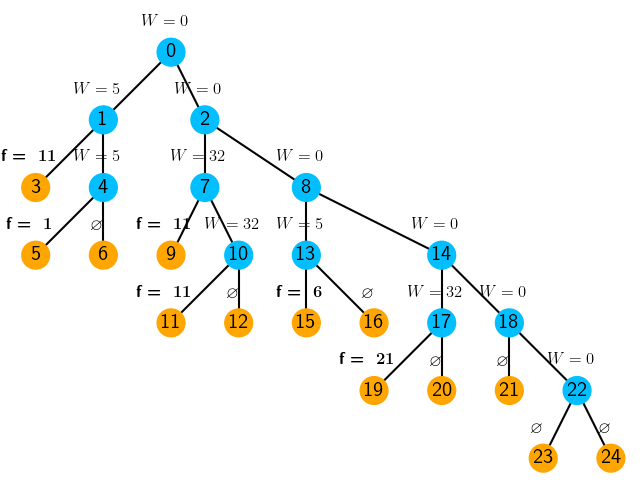
\includegraphics[scale=0.9]{brute_force_tree.png}
%   }
%   \caption{Решение задачи методом полного перебора}\label{fig:part2_brute_force_tree}
% \end{figure}

% \paragraph{Решение с помощью МВиГ.}

%  На рисунке \cref{fig:part2_branch_and_bound_tree} представлено дерево решения задачи методом ветвей и границ. Теперь закрытие вершины осуществляется в случаях:
%  \begin{itemize}
%    \item получен новый рекорд размещения;
%    \item оценка недопокрытия больше рекорда, полученного на предыдущих итерациях;
%    \item нет допустимого размещения БС.
% \end{itemize} 


% В таблице \cref{tab:branch_and_bound_solution} представлено решение МВиГ. Оптимальное решение получено на 5-ом узле дерева с недопокрытием $f(P)=1$. В ходе движения по дереву поиска, последующие оценки недопокрытия были больше полученного рекорда и данные вершины закрывались. В итоге общее количество узлов составило 16.


% \begin{figure}[ht]
%   \centerfloat{
%       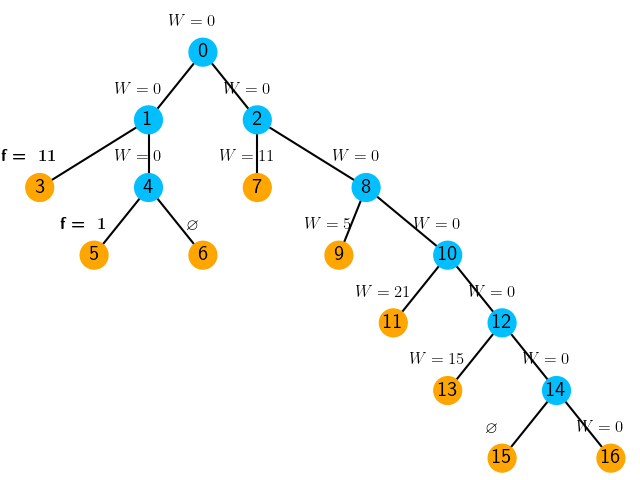
\includegraphics[scale=0.9]{branch_and_bound_tree.png}
%   }
%   \caption{Решение задачи методом ветвей и границ}\label{fig:part2_branch_and_bound_tree}
% \end{figure}

% \begin{table}[h!]\centering
%   \begin{tabular}{|c|c|c|}\hline
      
%       Oценка недопокрытия, $W(G_\nu)$ & Недопокрытие, $f(P)$ & Номер узла дерева, $\nu$\\
%       \hline
%       11 & Рекорд & 3\\
%       \textbf{1} & \textbf{Рекорд} & \textbf{5}\\
%       32 &  & 7\\
%       5 &  & 9\\
%       32 &  & 11\\
%       15 &  & 13\\
%       \hline

% \end{tabular}\caption{Решение полным перебором}\label{tab:branch_and_bound_solution}
% \end{table}


% \paragraph{Сравнение модели ЦЛП и комбинаторной модели}

% Теперь перейдем к решению задач большей размерности. Для различных случаев числа мест размещения $m$ и числа станций $n$ сравним результаты решения задачи представленными моделями. Оценка сравнения с помощью времени счета необъективна, так как алгоритм МВиГ и комбинаторная модель написаны на интерпретируемом языке Python. Коммерческие продукты представляют быстрые и качественные инструменты. Написание производительного кода для предложенных в данной диссертации моделей является отдельной не простой задачей, выходящей за рамки данного исследования. Коммерческие продукты решающие задачи ЦЛП основаны на алгоритме, предложенный Алисой Лэнд и Элисон Дойг \cite{Land1960}, в котором процедура поиска целочисленного решения также использует МВиГ.  Поэтому для сравнения моделей будет использована характеристика -- число просмотренных вершин в ходе поиска оптимального решения. Для сравнения также будут представлены решения задачи в комбинаторной форме методом полного перебора (МПП).

% Для каждого набора станций и мест размещения было рассчитано по 10 примеров с различными параметрами БС. В таблице \cref{tab:models_comparation}приводятся усредненные показатели числа просмотренных вершин дерева поиска по каждым 10 примерам. Результаты решения задачи максимизации покрытия влияют не только от количества точек размещения $n$, но также от их координат. Примем, что для каждой размерности для всех 10 примеров координаты фиксированные для всех моделей: МПП, МВиГ и ЦЛП. 


% \begin{table}
%   \caption{Результаты численного решения.}\label{tab:models_comparation}
%   \begin{tabular}{|ccc|*{3}{c}|} \cline{3-6}
%   \hline
%   \textbf{Число точек} & \textbf{Число} &\textbf{Количество} & \multicolumn{3}{c|}{\textbf{Количество пройденных}}\\ 
%   \textbf{размещения,} & \textbf{cтанций,} & \textbf{вариантов} & \multicolumn{3}{c|}{\textbf{узлов дерева поиска, $\nu$}}\\
%   \cline{4-6}
%   \textbf{$n$} & \textbf{$m$} &\textbf{размещения, $\gamma$} & \textbf{МПП}& \textbf{МВиГ} & \textbf{ЦЛП} \\ 
%   \hline
%   7 &  4 & 840 & 3122 & 360 &  \textbf{275} \\
%   7 &  5 & 2 520 & 16 114 & 560  &  \textbf{45}  \\
%   7 &  6 & 5 040 & 59 564 & 364  &  \textbf{19}  \\
%   8 &  4 & 1 680 &  4954 &  434 &   \textbf{189} \\
%   8 &  5 & 6 720 & 6720 & \textbf{852}  &  878 \\
%   8 &  6 & 20 160 &  15 9170 & 592  & \textbf{185}  \\
%   9  &  4 & 3 024 & 9 882 & \textbf{458} & 5511 \\
%   9  &  5 & 15 120&  58 190 &  \textbf{768} &  1236\\
%   9  &  6 & 60 480&  366 512 &  \textbf{720} & 13294 \\
%   10 &  4 & 5 040&  14 868&  \textbf{800}&  6243\\
%   10 &	5 & 30 240&  113 932&  \textbf{414}&  8043\\
%   10 &	6 & 151 200&  828 952&  \textbf{40 872}&  71587\\
%   11 &  4 & 7 920& 23 482&  \textbf{354} & 15538\\
%   11 &	5 & 55 440& 204 894& \textbf{9 138}&  74440\\
%   11 &	6 & 332 640& 1 592 500 & \textbf{88 002} & 413 767 \\
%   \hline
%   \end{tabular}
% \end{table} 

% Жирным цветом в колонках пройденных узлов в ходе движения по дереву поиска МПП, МВиГ и ЦЛП выделены минимальные значения для фиксированных значений $n$ и $m$ (размерностей задачи). Как видно из результатов сравнения, при увеличении размерности задачи разработанный алгоритм метода ветвей и границ для комбинаторной модели показывает лучшие результаты по сравнению с математической моделью ЦЛП.

\section{Выводы по главе 2}
Данная глава посвящена задачам оптимального размещения базовых станций в рамках комплексного проектирования беспроводных сетей связи. 
Спецификой моделей оптимизации является размещение станций для максимального телекоммуникационного покрытия вдоль протяженного объекта.

В главе были представлены следующие результаты:

\begin{enumerate}
  \item Представлена актуальность БШС с линейной топологией. Примерами таких сетей на месторождениях могут являться сети вдоль протяженных магистральных трубопроводов для организации связи как для сбора данных в составе АСУ ТП, а также организации высокоскоростной телекоммуникационной сети для сбора мультимедийного трафика с беспроводных камер видеонаблюдения. В рамках цифровизации месторождений набирает свой интерес задача внедрения современных высокоскоростных локальных сетей для мобильных обходчиков. Еще одним примером использования сетей с линейной топологии является организация телекоммуникационного покрытия вдоль промысловых автодорог для обеспечения безопасности обслуживающего персонала. 
  \item Представлена математическая модель задачи размещения станций в виде ЦЛП. Целевая функция модели представляет собой  суммарное телекоммуникационное покрытие участка, которое необходимо максимизировать. Также представлены ограничения равенства и неравенства модели, удовлетворяющие требованиями размещения -- обеспечение любой БС телекоммуникационной связью со шлюзами на концах участка через системы размещены станций и бюджетному ограничению стоимости размещения.
  \item Представлена математическая модель задачи размещения станций в виде экстремальной задачи в комбинаторной форме. Такой подход позволяет учитывать специфику конкретной задачи, что позволяет быстрее найти оптимальное решения. В такой постановке, в ходе поиска оптимального решение возможно проверять условие ограничения на время межконцевой задержки в сети, которое нелинейную зависимость от количества каналов в сети.
  \item Для решения комбинаторной модели задачи размещения предложен алгоритм типа ветвей и границ. Описана процедура построения бинарного дерева поиска, учитывающая специфику размещения множества станций $S$ на множества $A$ возможных точек размещения. Представлены различные модели оценки недопокрытия, необходимые для получения рекордов и возможности закрытия вершин дерева, для которых множество допустимых размещений пусто. Сравнительная оценка для частного случая размещения, когда необходимо разместить все имеющиеся станции показало, что с увеличением размерности задачи количество пройденных узлов комбинаторной модели существенно меньше чем в модели ЦЛП. 
  \item После нахождение оптимального решения на этапе синтеза топологии при проектировании БШС, полученное размещение попадает на этап математического моделирования, включающие в себя оценку различных характеристик сети, работу протокола, расчет надежности и т.д. В том случае, если проверка требований, предъявляемые к сети на этапе моделирования, проходит неуспешно, данное размещение становится невозможным. Для того чтобы  было возможно проверять не только оптимальное решение, но и размещения не хуже оптимального на заданное отклонение, было преложена процедура нахождения последовательности топологий сети для итерационной процедуры комплексного проектирования БШС. Процедура нахождения последовательности лучших решений задачи выбора и размещения базовых станций основана на разработанном алгоритме МВиГ.
  
\end{enumerate}



Результаты исследования, представленные в этой главе, были опубликованы в работах \cite{IvanovVAK2019, Ivanov2019, MukhtarovIvanovPershinDCCN2019_RSCI, Mukhtarov2020, VishnevskyMukhtarovPershinDCCN2020_RSCI, LazarevaLarionovMukhtarovITTMM2020_RSCI, VishnevskyLarionovMukhtarovICAM2020_RSCI, MukhtarovSokolovITTMM2021, PershinVAK2022}.  \fixme{Добавить астраханскую}.

% ============================================================
% Представлена математическая модель задачи размещения базовых станций беспроводной сети связи вдоль линейного участка в виде задачи ЦЛП. В качестве примера представлен численный пример решения задачи.


% В работе предложена методика проектирования беспроводной широкополосной сети для контроля линейной трассы с использованием итерационной процедуры построения последовательности лучших решений задачи выбора и размещения базовых станций при выполнении технологических условий на проектирование сети и ограничения на стоимость размещаемых станций. 

% Предложенная методика позволяет на этапе моделирования выбирать лучшее решение среди тех решений по выбору и размещению станций, которые удовлетворяют требованиям, предъявляемым к проектируемой сети.

% Процедура нахождения последовательности лучших решений задачи выбора и размещения базовых станций основана на разработанном алгоритме \fixme{МВиГ}.

% \fixme{
% Основным результатом работы, представленной в этой главе, является разработка итерационного метода выбора оптимальной топологии сети в процессе комплексного проектирования БШС. 
% Принципиальной особенностью предлагаемого метода, повышающей его эффективность, является то, что для рассмотрения на этапе моделирования предлагается не одно решения, а последовательности лучших решений задачи оптимизации топологии сети. Это позволяет с помощью разработанной итерационной процедуры выбирать на этапе моделирования лучшее решение среди тех решений по топологии, которые удовлетворяют требуемым характеристикам проектируемой БШС.} 

